\documentclass[11pt,a4paper]{scrartcl}
% =====================================================================
%  pds-apuntes.tex — Estilo común de apuntes y hojas de ejercicios.
%
%  Uso (desde teoría/Tx/apuntes/ o teoría/Tx/ejercicios/):
%     \documentclass[11pt,a4paper]{scrartcl}   % o scrreprt
%     % =====================================================================
%  pds-apuntes.tex — Estilo común de apuntes y hojas de ejercicios.
%
%  Uso (desde teoría/Tx/apuntes/ o teoría/Tx/ejercicios/):
%     \documentclass[11pt,a4paper]{scrartcl}   % o scrreprt
%     % =====================================================================
%  pds-apuntes.tex — Estilo común de apuntes y hojas de ejercicios.
%
%  Uso (desde teoría/Tx/apuntes/ o teoría/Tx/ejercicios/):
%     \documentclass[11pt,a4paper]{scrartcl}   % o scrreprt
%     \input{../../comun/pds-apuntes}
%     \tema{1}{Introducción: señales y sistemas}
%     \begin{document} \cabecera{Apuntes} ... \end{document}
%  Compilar con:  latexmk -xelatex  (o «make» desde teoría/)
% =====================================================================

\input{../../comun/pds-comun.tex}

\usepackage[a4paper, top=2.6cm, bottom=2.6cm, left=2.5cm, right=2.5cm,
            headheight=1.1cm]{geometry}
\usepackage{fontspec}
\usepackage{unicode-math}
\setmainfont{LibertinusSerif}[Extension=.otf, UprightFont=*-Regular, BoldFont=*-Semibold,
  ItalicFont=*-Italic, BoldItalicFont=*-SemiboldItalic]
\setsansfont{FiraSans}[Extension=.otf, UprightFont=*-Regular, BoldFont=*-SemiBold,
  ItalicFont=*-Italic, BoldItalicFont=*-SemiBoldItalic, Scale=MatchLowercase]
\setmonofont{FiraMono}[Extension=.otf, UprightFont=*-Regular, BoldFont=*-Medium, AutoFakeSlant=0.15, Scale=0.85]
\setmathfont{LibertinusMath-Regular.otf}

\usepackage{microtype}
\usepackage{enumitem}
\usepackage{multicol}
\setlist{itemsep=2pt, topsep=4pt}
\usepackage{caption}
\captionsetup{font=small, labelfont={sf,bf,color=pdsazul}, labelsep=period}
\usepackage{subcaption}
\usepackage[most]{tcolorbox}
\usepackage{environ}
\usepackage{scrlayer-scrpage}
\usepackage[hidelinks, unicode]{hyperref}
\usepackage[spanish, noabbrev]{cleveref}

% Títulos en Fira Sans con el azul de la asignatura
\setkomafont{disposition}{\sffamily\bfseries\color{pdsazul}}
\setkomafont{descriptionlabel}{\sffamily\bfseries}
\setlength{\parindent}{0pt}
\setlength{\parskip}{0.55\baselineskip plus 2pt}
\linespread{1.05}

% ---------------------------------------------------------------------
%  Datos del tema y cabeceras
% ---------------------------------------------------------------------
\newcommand{\numtema}{}
\newcommand{\nombretema}{}
\newcommand{\tema}[2]{\renewcommand{\numtema}{#1}\renewcommand{\nombretema}{#2}}

\pagestyle{scrheadings}
\clearpairofpagestyles
\ihead{\sffamily\small\color{pdsgris}\asignatura}
\ohead{\sffamily\small\color{pdsgris}Tema~\numtema. \nombretema}
\ifoot{\sffamily\small\color{pdsgris}\grado}
\ofoot{\sffamily\small\pagemark}
\setkomafont{pagehead}{\normalfont}
\setkomafont{pagefoot}{\normalfont}

% \cabecera{Apuntes|Ejercicios|...} : bloque de título de la primera página
\newcommand{\cabecera}[1]{%
  \thispagestyle{plain.scrheadings}%
  \noindent
  \begin{minipage}[c]{2.2cm}
    
\includegraphics[width=1.9cm]{../../comun/ucm.png}
  \end{minipage}%
  \begin{minipage}[c]{\dimexpr\linewidth-2.2cm}
    \sffamily
    {\small\color{pdsgris}\grado\par \asignatura\ · \curso\par}
    \vspace{4pt}
    {\Large\bfseries\color{pdsazul}#1\par}
    {\large\bfseries Tema~\numtema. \nombretema\par}
    \vspace{2pt}
    {\small\color{pdsgris}\autores\par}
  \end{minipage}\par
  \vspace{6pt}{\color{pdsazul}\rule{\linewidth}{0.8pt}}\par\vspace{4pt}}

% ---------------------------------------------------------------------
%  Cajas: definición, propiedad, ejemplo, nota, «en código»
% ---------------------------------------------------------------------
\tcbset{pdsbase/.style={enhanced, breakable, boxrule=0pt, arc=1.5pt, left=8pt, right=8pt,
    top=5pt, bottom=5pt, fonttitle=\sffamily\bfseries\small, coltitle=white,
    before skip=8pt, after skip=8pt}}
\newtcbtheorem[number within=section]{definicion}{Definición}%
  {pdsbase, colback=pdsfondo, colframe=pdsazul, borderline west={2.5pt}{0pt}{pdsazul}}{def}
\newtcbtheorem[use counter from=definicion]{propiedad}{Propiedad}%
  {pdsbase, colback=pdsfondo, colframe=pdsazul!75, borderline west={2.5pt}{0pt}{pdsazul!75}}{prop}
\newtcbtheorem[use counter from=definicion]{ejemplo}{Ejemplo}%
  {pdsbase, colback=pdsverde!5, colframe=pdsverde, borderline west={2.5pt}{0pt}{pdsverde}}{ej}
\newtcolorbox{nota}[1][Nota]{pdsbase, colback=pdsnaranja!7, colframe=pdsnaranja,
  title={#1}, borderline west={2.5pt}{0pt}{pdsnaranja}}
\newtcolorbox{importante}[1][Importante]{pdsbase, colback=pdsrojo!5, colframe=pdsrojo,
  title={#1}, borderline west={2.5pt}{0pt}{pdsrojo}}
\newtcolorbox{encodigo}[1][En código]{pdsbase, colback=white, colframe=pdsgris,
  title={#1}, borderline west={2.5pt}{0pt}{pdsgris}}

\lstset{basicstyle=\ttfamily\small}
\renewcommand{\codigoetiqueta}[1]{{\sffamily\small\bfseries\color{pdsgris}#1}}

% ---------------------------------------------------------------------
%  Hojas de ejercicios: \begin{ejercicio} ... \end{ejercicio} y
%  \begin{solucion} ... \end{solucion} (solo se imprime si se define
%  \SOLUCIONES antes de cargar el documento; ver *-Soluciones.tex)
% ---------------------------------------------------------------------
\newif\ifsoluciones
\ifdefined\SOLUCIONES \solucionestrue \fi
\newcounter{ejercicio}
\newenvironment{ejercicio}[1][]{%
  \refstepcounter{ejercicio}\par\vspace{6pt}%
  \noindent{\sffamily\bfseries\color{pdsazul}Ejercicio~\theejercicio}%
  \if\relax\detokenize{#1}\relax\else\ {\sffamily\color{pdsgris}(#1)}\fi\quad}%
  {\par}
\NewEnviron{solucion}{%
  \ifsoluciones
    \begin{tcolorbox}[pdsbase, colback=pdsverde!4, colframe=pdsverde,
      borderline west={2.5pt}{0pt}{pdsverde}, title={Solución}]
      \BODY
    \end{tcolorbox}
  \fi}
% \begin{incisos}[columnas] ... \end{incisos}: apartados a), b)... de un
% enunciado repartidos en columnas (3 por defecto)
% (con una sola columna no se usa multicols, que necesita al menos dos)
\newenvironment{incisos}[1][3]{\par\vspace{-2pt}%
  \ifnum#1>1 \def\finincisos{\end{multicols}}\begin{multicols}{#1}\raggedcolumns\raggedright
  \else\def\finincisos{}\fi
  \begin{enumerate}[label=\alph*), itemsep=3pt, topsep=0pt]}%
  {\end{enumerate}\finincisos\vspace{-4pt}}
\newcommand{\herramienta}[1]{\emph{Herramienta interactiva:} \texttt{herramientas/#1}}

%     \tema{1}{Introducción: señales y sistemas}
%     \begin{document} \cabecera{Apuntes} ... \end{document}
%  Compilar con:  latexmk -xelatex  (o «make» desde teoría/)
% =====================================================================

% =====================================================================
%  pds-comun.tex — Paquetes, colores y estilos de código comunes a
%  transparencias, apuntes y hojas de ejercicios. Compilar con XeLaTeX.
%  No cargar directamente: lo cargan pds-beamer.tex y pds-apuntes.tex.
% =====================================================================

\usepackage{polyglossia}
\setmainlanguage{spanish}
\usepackage{mathtools}
\usepackage{graphicx}
\usepackage{booktabs}
\usepackage{multirow}
\usepackage{array}
\usepackage{xcolor}
\usepackage{tikz}
\usetikzlibrary{positioning,arrows.meta,calc,shapes.geometric,decorations.pathreplacing}
\usepackage{listings}
\usepackage{siunitx}
\sisetup{output-decimal-marker={,}, group-separator={\,}, per-mode=symbol}

% Notas de erratas de versiones anteriores: no se imprimen salvo que se
% defina \ERRATAS antes de cargar el estilo (make ERRATAS=1)
\newif\iferratas
\ifdefined\ERRATAS \erratastrue \fi

% Ruta común (logo y figuras compartidas)
\providecommand{\rutacomun}{../../comun/}
\input{\rutacomun datos.tex}

% ---------------------------------------------------------------------
%  Paleta (la misma que usan las figuras generadas con Python,
%  ver comun/pds_estilo.py)
% ---------------------------------------------------------------------
\definecolor{pdsazul}{HTML}{2B3A8C}
\definecolor{pdsrojo}{HTML}{C0392B}
\definecolor{pdsverde}{HTML}{1E7B4F}
\definecolor{pdsnaranja}{HTML}{D9822B}
\definecolor{pdsgris}{HTML}{5A5A66}
\definecolor{pdsfondo}{HTML}{F3F4FA}
\definecolor{pdscodigo}{HTML}{F7F7F2}

% ---------------------------------------------------------------------
%  Diagramas de bloques (TikZ)
% ---------------------------------------------------------------------
\tikzset{
  bloque/.style={rectangle, rounded corners=2pt, draw=pdsazul!80, fill=pdsfondo,
                 very thick, minimum height=8mm, minimum width=14mm, align=center},
  sumador/.style={circle, draw=pdsazul!80, fill=pdsfondo, thick, inner sep=1.5pt},
  flecha/.style={-{Stealth[length=2.2mm]}, thick, pdsgris},
}

% ---------------------------------------------------------------------
%  Código: Python y Matlab en paralelo
% ---------------------------------------------------------------------
\newcommand{\pdscodesize}{\footnotesize}
\lstdefinestyle{pds}{
  basicstyle=\ttfamily\pdscodesize,
  keywordstyle=\color{pdsazul}\bfseries,
  commentstyle=\color{pdsverde}\itshape,
  stringstyle=\color{pdsrojo},
  numbers=none,
  backgroundcolor=\color{pdscodigo},
  frame=single, rulecolor=\color{pdsgris!40}, framerule=0.4pt,
  xleftmargin=2pt, xrightmargin=2pt, aboveskip=2pt, belowskip=2pt,
  columns=fullflexible, keepspaces=true,
  showstringspaces=false, breaklines=true, tabsize=4,
  upquote=true,
  % Con XeLaTeX, listings desordena los caracteres no ASCII junto a
  % dígitos («2π» sale «π2»): se sustituyen por su versión matemática.
  literate={π}{{$\pi$}}1 {δ}{{$\delta$}}1 {ω}{{$\omega$}}1 {Ω}{{$\Omega$}}1
           {≈}{{$\approx$}}1 {µ}{{$\mu$}}1 {·}{{$\cdot$}}1 {α}{{$\alpha$}}1
           {á}{{á}}1 {é}{{é}}1 {í}{{í}}1 {ó}{{ó}}1 {ú}{{ú}}1 {ñ}{{ñ}}1 {¿}{{¿}}1,
}
\lstdefinestyle{python}{style=pds, language=Python,
  morekeywords={as,True,False,None}}
\lstdefinestyle{matlab}{style=pds, language=Matlab,
  morekeywords={function,end,true,false}}

% \codigo{<ruta sin extensión>} muestra el mismo ejemplo en Python
% y en Matlab, uno al lado del otro. Los ficheros viven en
% ../codigo/python/<nombre>.py y ../codigo/matlab/<nombre>.m y se
% ejecutan en las pruebas (make prueba-codigo).
\newcommand{\rutacodigo}{../codigo/}
\newcommand{\codigoetiqueta}[1]{{\sffamily\scriptsize\bfseries\color{pdsgris}#1}}
\newcommand{\codigo}[2][]{%
  \par\noindent
  \begin{minipage}[t]{0.495\linewidth}
    \codigoetiqueta{Python}\par\vspace{1pt}
    \lstinputlisting[style=python,#1]{\rutacodigo python/#2.py}
  \end{minipage}\hfill
  \begin{minipage}[t]{0.495\linewidth}
    \codigoetiqueta{Matlab}\par\vspace{1pt}
    \lstinputlisting[style=matlab,#1]{\rutacodigo matlab/#2.m}
  \end{minipage}\par}

\input{\rutacomun notacion.tex}


\usepackage[a4paper, top=2.6cm, bottom=2.6cm, left=2.5cm, right=2.5cm,
            headheight=1.1cm]{geometry}
\usepackage{fontspec}
\usepackage{unicode-math}
\setmainfont{LibertinusSerif}[Extension=.otf, UprightFont=*-Regular, BoldFont=*-Semibold,
  ItalicFont=*-Italic, BoldItalicFont=*-SemiboldItalic]
\setsansfont{FiraSans}[Extension=.otf, UprightFont=*-Regular, BoldFont=*-SemiBold,
  ItalicFont=*-Italic, BoldItalicFont=*-SemiBoldItalic, Scale=MatchLowercase]
\setmonofont{FiraMono}[Extension=.otf, UprightFont=*-Regular, BoldFont=*-Medium, AutoFakeSlant=0.15, Scale=0.85]
\setmathfont{LibertinusMath-Regular.otf}

\usepackage{microtype}
\usepackage{enumitem}
\usepackage{multicol}
\setlist{itemsep=2pt, topsep=4pt}
\usepackage{caption}
\captionsetup{font=small, labelfont={sf,bf,color=pdsazul}, labelsep=period}
\usepackage{subcaption}
\usepackage[most]{tcolorbox}
\usepackage{environ}
\usepackage{scrlayer-scrpage}
\usepackage[hidelinks, unicode]{hyperref}
\usepackage[spanish, noabbrev]{cleveref}

% Títulos en Fira Sans con el azul de la asignatura
\setkomafont{disposition}{\sffamily\bfseries\color{pdsazul}}
\setkomafont{descriptionlabel}{\sffamily\bfseries}
\setlength{\parindent}{0pt}
\setlength{\parskip}{0.55\baselineskip plus 2pt}
\linespread{1.05}

% ---------------------------------------------------------------------
%  Datos del tema y cabeceras
% ---------------------------------------------------------------------
\newcommand{\numtema}{}
\newcommand{\nombretema}{}
\newcommand{\tema}[2]{\renewcommand{\numtema}{#1}\renewcommand{\nombretema}{#2}}

\pagestyle{scrheadings}
\clearpairofpagestyles
\ihead{\sffamily\small\color{pdsgris}\asignatura}
\ohead{\sffamily\small\color{pdsgris}Tema~\numtema. \nombretema}
\ifoot{\sffamily\small\color{pdsgris}\grado}
\ofoot{\sffamily\small\pagemark}
\setkomafont{pagehead}{\normalfont}
\setkomafont{pagefoot}{\normalfont}

% \cabecera{Apuntes|Ejercicios|...} : bloque de título de la primera página
\newcommand{\cabecera}[1]{%
  \thispagestyle{plain.scrheadings}%
  \noindent
  \begin{minipage}[c]{2.2cm}
    
\includegraphics[width=1.9cm]{../../comun/ucm.png}
  \end{minipage}%
  \begin{minipage}[c]{\dimexpr\linewidth-2.2cm}
    \sffamily
    {\small\color{pdsgris}\grado\par \asignatura\ · \curso\par}
    \vspace{4pt}
    {\Large\bfseries\color{pdsazul}#1\par}
    {\large\bfseries Tema~\numtema. \nombretema\par}
    \vspace{2pt}
    {\small\color{pdsgris}\autores\par}
  \end{minipage}\par
  \vspace{6pt}{\color{pdsazul}\rule{\linewidth}{0.8pt}}\par\vspace{4pt}}

% ---------------------------------------------------------------------
%  Cajas: definición, propiedad, ejemplo, nota, «en código»
% ---------------------------------------------------------------------
\tcbset{pdsbase/.style={enhanced, breakable, boxrule=0pt, arc=1.5pt, left=8pt, right=8pt,
    top=5pt, bottom=5pt, fonttitle=\sffamily\bfseries\small, coltitle=white,
    before skip=8pt, after skip=8pt}}
\newtcbtheorem[number within=section]{definicion}{Definición}%
  {pdsbase, colback=pdsfondo, colframe=pdsazul, borderline west={2.5pt}{0pt}{pdsazul}}{def}
\newtcbtheorem[use counter from=definicion]{propiedad}{Propiedad}%
  {pdsbase, colback=pdsfondo, colframe=pdsazul!75, borderline west={2.5pt}{0pt}{pdsazul!75}}{prop}
\newtcbtheorem[use counter from=definicion]{ejemplo}{Ejemplo}%
  {pdsbase, colback=pdsverde!5, colframe=pdsverde, borderline west={2.5pt}{0pt}{pdsverde}}{ej}
\newtcolorbox{nota}[1][Nota]{pdsbase, colback=pdsnaranja!7, colframe=pdsnaranja,
  title={#1}, borderline west={2.5pt}{0pt}{pdsnaranja}}
\newtcolorbox{importante}[1][Importante]{pdsbase, colback=pdsrojo!5, colframe=pdsrojo,
  title={#1}, borderline west={2.5pt}{0pt}{pdsrojo}}
\newtcolorbox{encodigo}[1][En código]{pdsbase, colback=white, colframe=pdsgris,
  title={#1}, borderline west={2.5pt}{0pt}{pdsgris}}

\lstset{basicstyle=\ttfamily\small}
\renewcommand{\codigoetiqueta}[1]{{\sffamily\small\bfseries\color{pdsgris}#1}}

% ---------------------------------------------------------------------
%  Hojas de ejercicios: \begin{ejercicio} ... \end{ejercicio} y
%  \begin{solucion} ... \end{solucion} (solo se imprime si se define
%  \SOLUCIONES antes de cargar el documento; ver *-Soluciones.tex)
% ---------------------------------------------------------------------
\newif\ifsoluciones
\ifdefined\SOLUCIONES \solucionestrue \fi
\newcounter{ejercicio}
\newenvironment{ejercicio}[1][]{%
  \refstepcounter{ejercicio}\par\vspace{6pt}%
  \noindent{\sffamily\bfseries\color{pdsazul}Ejercicio~\theejercicio}%
  \if\relax\detokenize{#1}\relax\else\ {\sffamily\color{pdsgris}(#1)}\fi\quad}%
  {\par}
\NewEnviron{solucion}{%
  \ifsoluciones
    \begin{tcolorbox}[pdsbase, colback=pdsverde!4, colframe=pdsverde,
      borderline west={2.5pt}{0pt}{pdsverde}, title={Solución}]
      \BODY
    \end{tcolorbox}
  \fi}
% \begin{incisos}[columnas] ... \end{incisos}: apartados a), b)... de un
% enunciado repartidos en columnas (3 por defecto)
% (con una sola columna no se usa multicols, que necesita al menos dos)
\newenvironment{incisos}[1][3]{\par\vspace{-2pt}%
  \ifnum#1>1 \def\finincisos{\end{multicols}}\begin{multicols}{#1}\raggedcolumns\raggedright
  \else\def\finincisos{}\fi
  \begin{enumerate}[label=\alph*), itemsep=3pt, topsep=0pt]}%
  {\end{enumerate}\finincisos\vspace{-4pt}}
\newcommand{\herramienta}[1]{\emph{Herramienta interactiva:} \texttt{herramientas/#1}}

%     \tema{1}{Introducción: señales y sistemas}
%     \begin{document} \cabecera{Apuntes} ... \end{document}
%  Compilar con:  latexmk -xelatex  (o «make» desde teoría/)
% =====================================================================

% =====================================================================
%  pds-comun.tex — Paquetes, colores y estilos de código comunes a
%  transparencias, apuntes y hojas de ejercicios. Compilar con XeLaTeX.
%  No cargar directamente: lo cargan pds-beamer.tex y pds-apuntes.tex.
% =====================================================================

\usepackage{polyglossia}
\setmainlanguage{spanish}
\usepackage{mathtools}
\usepackage{graphicx}
\usepackage{booktabs}
\usepackage{multirow}
\usepackage{array}
\usepackage{xcolor}
\usepackage{tikz}
\usetikzlibrary{positioning,arrows.meta,calc,shapes.geometric,decorations.pathreplacing}
\usepackage{listings}
\usepackage{siunitx}
\sisetup{output-decimal-marker={,}, group-separator={\,}, per-mode=symbol}

% Notas de erratas de versiones anteriores: no se imprimen salvo que se
% defina \ERRATAS antes de cargar el estilo (make ERRATAS=1)
\newif\iferratas
\ifdefined\ERRATAS \erratastrue \fi

% Ruta común (logo y figuras compartidas)
\providecommand{\rutacomun}{../../comun/}
\input{\rutacomun datos.tex}

% ---------------------------------------------------------------------
%  Paleta (la misma que usan las figuras generadas con Python,
%  ver comun/pds_estilo.py)
% ---------------------------------------------------------------------
\definecolor{pdsazul}{HTML}{2B3A8C}
\definecolor{pdsrojo}{HTML}{C0392B}
\definecolor{pdsverde}{HTML}{1E7B4F}
\definecolor{pdsnaranja}{HTML}{D9822B}
\definecolor{pdsgris}{HTML}{5A5A66}
\definecolor{pdsfondo}{HTML}{F3F4FA}
\definecolor{pdscodigo}{HTML}{F7F7F2}

% ---------------------------------------------------------------------
%  Diagramas de bloques (TikZ)
% ---------------------------------------------------------------------
\tikzset{
  bloque/.style={rectangle, rounded corners=2pt, draw=pdsazul!80, fill=pdsfondo,
                 very thick, minimum height=8mm, minimum width=14mm, align=center},
  sumador/.style={circle, draw=pdsazul!80, fill=pdsfondo, thick, inner sep=1.5pt},
  flecha/.style={-{Stealth[length=2.2mm]}, thick, pdsgris},
}

% ---------------------------------------------------------------------
%  Código: Python y Matlab en paralelo
% ---------------------------------------------------------------------
\newcommand{\pdscodesize}{\footnotesize}
\lstdefinestyle{pds}{
  basicstyle=\ttfamily\pdscodesize,
  keywordstyle=\color{pdsazul}\bfseries,
  commentstyle=\color{pdsverde}\itshape,
  stringstyle=\color{pdsrojo},
  numbers=none,
  backgroundcolor=\color{pdscodigo},
  frame=single, rulecolor=\color{pdsgris!40}, framerule=0.4pt,
  xleftmargin=2pt, xrightmargin=2pt, aboveskip=2pt, belowskip=2pt,
  columns=fullflexible, keepspaces=true,
  showstringspaces=false, breaklines=true, tabsize=4,
  upquote=true,
  % Con XeLaTeX, listings desordena los caracteres no ASCII junto a
  % dígitos («2π» sale «π2»): se sustituyen por su versión matemática.
  literate={π}{{$\pi$}}1 {δ}{{$\delta$}}1 {ω}{{$\omega$}}1 {Ω}{{$\Omega$}}1
           {≈}{{$\approx$}}1 {µ}{{$\mu$}}1 {·}{{$\cdot$}}1 {α}{{$\alpha$}}1
           {á}{{á}}1 {é}{{é}}1 {í}{{í}}1 {ó}{{ó}}1 {ú}{{ú}}1 {ñ}{{ñ}}1 {¿}{{¿}}1,
}
\lstdefinestyle{python}{style=pds, language=Python,
  morekeywords={as,True,False,None}}
\lstdefinestyle{matlab}{style=pds, language=Matlab,
  morekeywords={function,end,true,false}}

% \codigo{<ruta sin extensión>} muestra el mismo ejemplo en Python
% y en Matlab, uno al lado del otro. Los ficheros viven en
% ../codigo/python/<nombre>.py y ../codigo/matlab/<nombre>.m y se
% ejecutan en las pruebas (make prueba-codigo).
\newcommand{\rutacodigo}{../codigo/}
\newcommand{\codigoetiqueta}[1]{{\sffamily\scriptsize\bfseries\color{pdsgris}#1}}
\newcommand{\codigo}[2][]{%
  \par\noindent
  \begin{minipage}[t]{0.495\linewidth}
    \codigoetiqueta{Python}\par\vspace{1pt}
    \lstinputlisting[style=python,#1]{\rutacodigo python/#2.py}
  \end{minipage}\hfill
  \begin{minipage}[t]{0.495\linewidth}
    \codigoetiqueta{Matlab}\par\vspace{1pt}
    \lstinputlisting[style=matlab,#1]{\rutacodigo matlab/#2.m}
  \end{minipage}\par}

\input{\rutacomun notacion.tex}


\usepackage[a4paper, top=2.6cm, bottom=2.6cm, left=2.5cm, right=2.5cm,
            headheight=1.1cm]{geometry}
\usepackage{fontspec}
\usepackage{unicode-math}
\setmainfont{LibertinusSerif}[Extension=.otf, UprightFont=*-Regular, BoldFont=*-Semibold,
  ItalicFont=*-Italic, BoldItalicFont=*-SemiboldItalic]
\setsansfont{FiraSans}[Extension=.otf, UprightFont=*-Regular, BoldFont=*-SemiBold,
  ItalicFont=*-Italic, BoldItalicFont=*-SemiBoldItalic, Scale=MatchLowercase]
\setmonofont{FiraMono}[Extension=.otf, UprightFont=*-Regular, BoldFont=*-Medium, AutoFakeSlant=0.15, Scale=0.85]
\setmathfont{LibertinusMath-Regular.otf}

\usepackage{microtype}
\usepackage{enumitem}
\usepackage{multicol}
\setlist{itemsep=2pt, topsep=4pt}
\usepackage{caption}
\captionsetup{font=small, labelfont={sf,bf,color=pdsazul}, labelsep=period}
\usepackage{subcaption}
\usepackage[most]{tcolorbox}
\usepackage{environ}
\usepackage{scrlayer-scrpage}
\usepackage[hidelinks, unicode]{hyperref}
\usepackage[spanish, noabbrev]{cleveref}

% Títulos en Fira Sans con el azul de la asignatura
\setkomafont{disposition}{\sffamily\bfseries\color{pdsazul}}
\setkomafont{descriptionlabel}{\sffamily\bfseries}
\setlength{\parindent}{0pt}
\setlength{\parskip}{0.55\baselineskip plus 2pt}
\linespread{1.05}

% ---------------------------------------------------------------------
%  Datos del tema y cabeceras
% ---------------------------------------------------------------------
\newcommand{\numtema}{}
\newcommand{\nombretema}{}
\newcommand{\tema}[2]{\renewcommand{\numtema}{#1}\renewcommand{\nombretema}{#2}}

\pagestyle{scrheadings}
\clearpairofpagestyles
\ihead{\sffamily\small\color{pdsgris}\asignatura}
\ohead{\sffamily\small\color{pdsgris}Tema~\numtema. \nombretema}
\ifoot{\sffamily\small\color{pdsgris}\grado}
\ofoot{\sffamily\small\pagemark}
\setkomafont{pagehead}{\normalfont}
\setkomafont{pagefoot}{\normalfont}

% \cabecera{Apuntes|Ejercicios|...} : bloque de título de la primera página
\newcommand{\cabecera}[1]{%
  \thispagestyle{plain.scrheadings}%
  \noindent
  \begin{minipage}[c]{2.2cm}
    
\includegraphics[width=1.9cm]{../../comun/ucm.png}
  \end{minipage}%
  \begin{minipage}[c]{\dimexpr\linewidth-2.2cm}
    \sffamily
    {\small\color{pdsgris}\grado\par \asignatura\ · \curso\par}
    \vspace{4pt}
    {\Large\bfseries\color{pdsazul}#1\par}
    {\large\bfseries Tema~\numtema. \nombretema\par}
    \vspace{2pt}
    {\small\color{pdsgris}\autores\par}
  \end{minipage}\par
  \vspace{6pt}{\color{pdsazul}\rule{\linewidth}{0.8pt}}\par\vspace{4pt}}

% ---------------------------------------------------------------------
%  Cajas: definición, propiedad, ejemplo, nota, «en código»
% ---------------------------------------------------------------------
\tcbset{pdsbase/.style={enhanced, breakable, boxrule=0pt, arc=1.5pt, left=8pt, right=8pt,
    top=5pt, bottom=5pt, fonttitle=\sffamily\bfseries\small, coltitle=white,
    before skip=8pt, after skip=8pt}}
\newtcbtheorem[number within=section]{definicion}{Definición}%
  {pdsbase, colback=pdsfondo, colframe=pdsazul, borderline west={2.5pt}{0pt}{pdsazul}}{def}
\newtcbtheorem[use counter from=definicion]{propiedad}{Propiedad}%
  {pdsbase, colback=pdsfondo, colframe=pdsazul!75, borderline west={2.5pt}{0pt}{pdsazul!75}}{prop}
\newtcbtheorem[use counter from=definicion]{ejemplo}{Ejemplo}%
  {pdsbase, colback=pdsverde!5, colframe=pdsverde, borderline west={2.5pt}{0pt}{pdsverde}}{ej}
\newtcolorbox{nota}[1][Nota]{pdsbase, colback=pdsnaranja!7, colframe=pdsnaranja,
  title={#1}, borderline west={2.5pt}{0pt}{pdsnaranja}}
\newtcolorbox{importante}[1][Importante]{pdsbase, colback=pdsrojo!5, colframe=pdsrojo,
  title={#1}, borderline west={2.5pt}{0pt}{pdsrojo}}
\newtcolorbox{encodigo}[1][En código]{pdsbase, colback=white, colframe=pdsgris,
  title={#1}, borderline west={2.5pt}{0pt}{pdsgris}}

\lstset{basicstyle=\ttfamily\small}
\renewcommand{\codigoetiqueta}[1]{{\sffamily\small\bfseries\color{pdsgris}#1}}

% ---------------------------------------------------------------------
%  Hojas de ejercicios: \begin{ejercicio} ... \end{ejercicio} y
%  \begin{solucion} ... \end{solucion} (solo se imprime si se define
%  \SOLUCIONES antes de cargar el documento; ver *-Soluciones.tex)
% ---------------------------------------------------------------------
\newif\ifsoluciones
\ifdefined\SOLUCIONES \solucionestrue \fi
\newcounter{ejercicio}
\newenvironment{ejercicio}[1][]{%
  \refstepcounter{ejercicio}\par\vspace{6pt}%
  \noindent{\sffamily\bfseries\color{pdsazul}Ejercicio~\theejercicio}%
  \if\relax\detokenize{#1}\relax\else\ {\sffamily\color{pdsgris}(#1)}\fi\quad}%
  {\par}
\NewEnviron{solucion}{%
  \ifsoluciones
    \begin{tcolorbox}[pdsbase, colback=pdsverde!4, colframe=pdsverde,
      borderline west={2.5pt}{0pt}{pdsverde}, title={Solución}]
      \BODY
    \end{tcolorbox}
  \fi}
% \begin{incisos}[columnas] ... \end{incisos}: apartados a), b)... de un
% enunciado repartidos en columnas (3 por defecto)
% (con una sola columna no se usa multicols, que necesita al menos dos)
\newenvironment{incisos}[1][3]{\par\vspace{-2pt}%
  \ifnum#1>1 \def\finincisos{\end{multicols}}\begin{multicols}{#1}\raggedcolumns\raggedright
  \else\def\finincisos{}\fi
  \begin{enumerate}[label=\alph*), itemsep=3pt, topsep=0pt]}%
  {\end{enumerate}\finincisos\vspace{-4pt}}
\newcommand{\herramienta}[1]{\emph{Herramienta interactiva:} \texttt{herramientas/#1}}

\graphicspath{{../figuras/}}
\tema{2}{Muestreo y reconstrucción de señales}
\renewcommand{\rutacodigo}{../codigo/}

\hypersetup{pdftitle={Tema 2. Muestreo y reconstrucción de señales},
  pdfauthor={\autores}}

\begin{document}
\cabecera{Apuntes}

\begin{nota}[Cómo usar estos apuntes]
  Estos apuntes desarrollan el contenido de las cuatro presentaciones del tema: las secciones~\ref{sec:intro}–\ref{sec:teorema} corresponden a la parte~1 (muestreo y aliasing), la sección~\ref{sec:reconstruccion} a la parte~2 (reconstrucción), la sección~\ref{sec:cuantificacion} a la parte~3 (cuantificación y codificación) y la sección~\ref{sec:discreto} a la parte~4 (muestreo de señales discretas). Los ejemplos de código están en \texttt{teoría/T2/codigo/}, en Python y en Matlab, y se pueden ejecutar tal cual. Al final de cada sección se indican los ejercicios de la hoja del tema que la practican.
\end{nota}

\tableofcontents

% =====================================================================
\section{Del mundo analógico al digital}\label{sec:intro}

Casi todas las señales que interesa procesar son analógicas: la presión acústica, la tensión de un electrodo, la temperatura o el campo electromagnético que recibe una antena. Durante buena parte del siglo~XX se procesaron con circuitos analógicos: el predictor de mareas de Lord Kelvin (1873) sumaba sinusoides con poleas y engranajes, y desde los años cuarenta los amplificadores operacionales permitieron construir sumadores, integradores y filtros. Son rápidos, pero sensibles al ruido y a la deriva de los componentes, y poco flexibles: cambiar el procesado exige cambiar el circuito.

El procesado digital sustituye el circuito por un programa. Su despegue se apoya en tres hitos: el algoritmo FFT de Cooley y Tukey (1965), que hizo práctico calcular espectros (Gauss había usado una idea equivalente hacia 1805), el Intel~2920 (1979), un procesador de señal con conversores integrados, y el TMS32010 de Texas Instruments (1983), el primer DSP de éxito comercial, con arquitectura Harvard y una instrucción de multiplicar y acumular en un ciclo.

\subsection{La cadena de procesado}

Para procesar digitalmente una señal analógica se sigue la cadena de la \cref{fig:cadena}. El filtro antialiasing limita el ancho de banda de la entrada; el conversor A/D la \emph{muestrea} (toma valores en instantes discretos), la \emph{cuantifica} (redondea cada valor a uno de un conjunto finito) y la \emph{codifica} (asigna a cada valor una palabra binaria). El procesador opera sobre la secuencia de números y, si la salida tiene que volver a ser analógica, el conversor D/A y el filtro de suavizado la reconstruyen.

\begin{figure}[ht]
  \centering
  \resizebox{\linewidth}{!}{%
  \begin{tikzpicture}[node distance=0.9cm]
    \node (x) {$x_a(t)$};
    \node[bloque, right=of x] (aa) {Filtro\\antialiasing};
    \node[bloque, right=of aa] (ad) {A/D};
    \node[bloque, right=of ad, fill=pdsazul!12] (dsp) {Procesado\\digital};
    \node[bloque, right=of dsp] (da) {D/A};
    \node[bloque, right=of da] (rec) {Filtro de\\suavizado};
    \node[right=of rec] (y) {$y_a(t)$};
    \draw[flecha] (x) -- (aa); \draw[flecha] (aa) -- (ad);
    \draw[flecha] (ad) -- node[above, font=\footnotesize]{$x[n]$} (dsp);
    \draw[flecha] (dsp) -- node[above, font=\footnotesize]{$y[n]$} (da);
    \draw[flecha] (da) -- (rec); \draw[flecha] (rec) -- (y);
  \end{tikzpicture}}
  \caption{Cadena de procesado digital de una señal analógica.}
  \label{fig:cadena}
\end{figure}

La \cref{fig:mcc} muestra los tres pasos de la conversión A/D. Cada uno introduce un tipo de error distinto, y este tema estudia cuándo y cuánto:
\begin{itemize}
  \item El \textbf{muestreo} no pierde información si la señal tiene banda limitada y se muestrea lo bastante deprisa (\cref{sec:muestreo,sec:teorema}). Si no, aparece el \emph{aliasing}.
  \item La \textbf{reconstrucción} ideal recupera la señal exactamente, pero no es realizable; los retenedores la aproximan (\cref{sec:reconstruccion}).
  \item La \textbf{cuantificación} siempre pierde información, pero el error se puede hacer tan pequeño como se quiera añadiendo bits (\cref{sec:cuantificacion}).
\end{itemize}

\begin{figure}[ht]
  \centering
  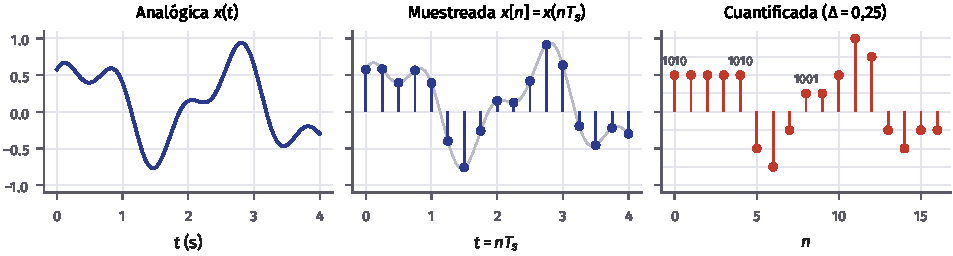
\includegraphics[width=0.9\linewidth]{muestreo_cuant_cod}
  \caption{Señal analógica, señal muestreada (tiempo discreto, amplitud continua) y señal cuantificada (digital).}
  \label{fig:mcc}
\end{figure}

% =====================================================================
\section{Muestreo periódico y aliasing}\label{sec:muestreo}

\begin{definicion}{Muestreo periódico}{muestreo}
  Muestrear periódicamente una señal $x(t)$ con \emph{periodo de muestreo} $T_s$ es formar la secuencia
  \[
    x[n]=x(nT_s),\qquad n\in\Z.
  \]
  La \emph{frecuencia de muestreo} es $f_s=1/T_s$ en Hz, o $\omega_s=2\pi f_s=2\pi/T_s$ en rad/s.
\end{definicion}

La secuencia no guarda $T_s$: es una lista de números. Los mismos números representan una señal lenta muestreada despacio o una rápida muestreada deprisa, y solo al conocer $T_s$ (o $f_s$) se puede volver a la escala de tiempo física (\cref{fig:muestreo}).

\begin{figure}[ht]
  \centering
  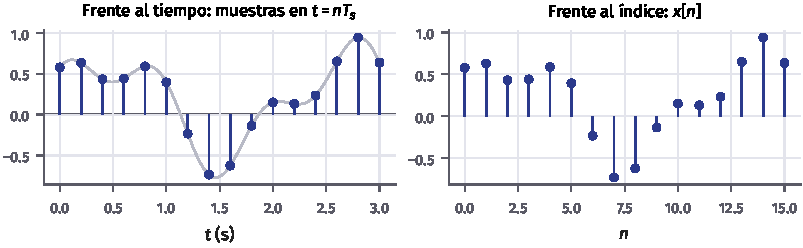
\includegraphics[width=0.7\linewidth]{muestreo_periodico}
  \caption{Muestreo periódico de una señal continua.}
  \label{fig:muestreo}
\end{figure}

\subsection{Frecuencia continua y frecuencia discreta}

Si se muestrea una sinusoide $x(t)=A\cos(\omega_0t+\phi)$, se obtiene
\[
  x[n]=A\cos(\omega_0T_sn+\phi)=A\cos(\Omega_0n+\phi),\qquad
  \Omega_0=\omega_0T_s=2\pi\frac{f_0}{f_s}.
\]
La frecuencia discreta $\Omega$ (rad/muestra) es la frecuencia continua $\omega$ (rad/s) \emph{normalizada} por la frecuencia de muestreo. En ciclos por muestra, $F_0=f_0/f_s$. Esta relación,
\begin{equation}\label{eq:omega}
  \boxed{\Omega=\omega T_s=\frac{2\pi\omega}{\omega_s}}
\end{equation}
es la clave de todo el tema y la que permite traducir especificaciones en hercios a frecuencias discretas y viceversa.

\begin{ejemplo}{Una frecuencia en tres unidades}{unidades}
  Un tono de $f_0=1$\,kHz muestreado a $f_s=8$\,kHz tiene $\omega_0=2000\pi$\,rad/s, $F_0=1/8$ ciclos por muestra y $\Omega_0=\pi/4$\,rad/muestra: cada periodo del tono ocupa ocho muestras. Si el mismo tono se muestrea a $f_s=48$\,kHz, $\Omega_0=\pi/24$.
\end{ejemplo}

\subsection{Alias}

En el Tema~1 vimos que las frecuencias discretas $\Omega_0$ y $\Omega_0+2\pi k$ dan la misma secuencia, porque $\e^{j2\pi kn}=1$. Deshaciendo el cambio \eqref{eq:omega}, todas las frecuencias continuas
\[
  \omega_k=\omega_0+k\,\omega_s,\qquad k\in\Z,
\]
producen exactamente las mismas muestras. Como el coseno es par, también $-\omega_0+k\omega_s$. Cada una de estas sinusoides es un \emph{alias} de las demás: al muestrear se vuelven indistinguibles (\cref{fig:alias}).

\begin{figure}[ht]
  \centering
  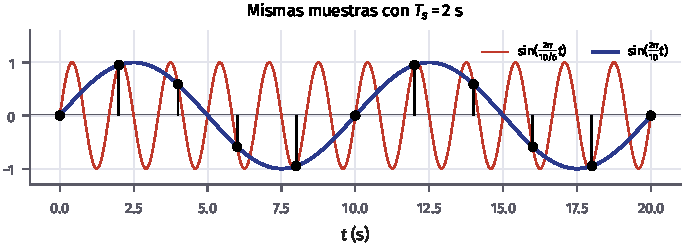
\includegraphics[width=0.8\linewidth]{alias_sinusoides}
  \caption{Dos sinusoides de frecuencias distintas que dan las mismas muestras.}
  \label{fig:alias}
\end{figure}

\begin{definicion}{Alias fundamental}{alias}
  El \emph{alias fundamental} de una sinusoide muestreada es el de menor frecuencia: el único con $\abs{\Omega}\le\pi$ o, lo que es lo mismo, con $\abs{\omega}\le\omega_s/2$. Se obtiene llevando $\Omega_0$ al intervalo $[-\pi,\pi)$ con
  \[
    \Omega_a=\big((\Omega_0+\pi)\bmod 2\pi\big)-\pi.
  \]
\end{definicion}

Si la sinusoide original cumple $\abs{\omega_0}<\omega_s/2$, ella misma es el alias fundamental y no hay ambigüedad. Si no, existe una sinusoide de frecuencia menor con las mismas muestras y cualquier reconstrucción que produzca señales de frecuencia menor que $\omega_s/2$ devolverá esa y no la original. Este fenómeno se llama \emph{aliasing} (en castellano, a veces, solapamiento).

En hercios, una sinusoide de frecuencia $f_0$ aparece en la \emph{frecuencia aparente}
\[
  f_a=\abs{f_0-kf_s}\in[0,f_s/2],\qquad k=\text{el entero más próximo a }f_0/f_s.
\]
El eje de frecuencias «se pliega» en los múltiplos de $f_s/2$, que se llama \emph{frecuencia de Nyquist} (\cref{fig:alias-mapa}). Es lo que hace que las ruedas de un coche parezcan girar despacio o al revés en un vídeo, o que un tono de 30\,kHz grabado a 48\,kHz sin filtrar suene a 18\,kHz.

\begin{figure}[ht]
  \centering
  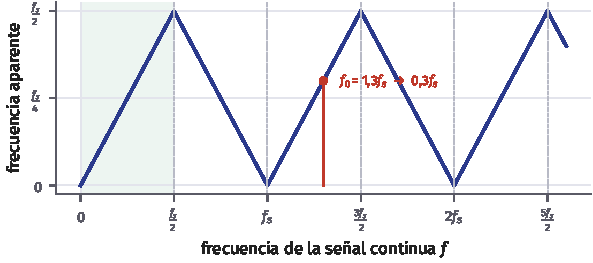
\includegraphics[width=0.6\linewidth]{alias_mapa}
  \caption{Frecuencia aparente en función de la frecuencia de la sinusoide muestreada.}
  \label{fig:alias-mapa}
\end{figure}

\begin{ejemplo}{Alias de una sinusoide y de una suma}{alias}
  Con $T_s=2$\,s:
  \begin{itemize}
    \item $\sin\big(\frac{2\pi}{10}t\big)$ tiene $\Omega_0=\frac{4\pi}{10}<\pi$: ya es su alias fundamental.
    \item $\sin\big(\frac{2\pi}{10/6}t\big)$ tiene $\Omega_0=\frac{24\pi}{10}$. Restando $2\pi$, $\Omega_a=\frac{4\pi}{10}$, que corresponde a $\omega=\Omega_a/T_s=\frac{2\pi}{10}$\,rad/s. Las dos señales dan las mismas muestras.
    \item $x(t)=3\sin\big(\frac{2\pi}{5}t\big)+\sin\big(\frac{2\pi}{3}t\big)$: el primer término tiene $\Omega_1=\frac{4\pi}{5}<\pi$ y se conserva; el segundo, $\Omega_2=\frac{4\pi}{3}$, que se pliega a $\frac{4\pi}{3}-2\pi=-\frac{2\pi}{3}$, es decir, $\omega=-\frac{\pi}{3}$\,rad/s. Como el seno es impar, el alias fundamental es
    \[
      3\sin\big(\tfrac{2\pi}{5}t\big)-\sin\big(\tfrac{\pi}{3}t\big).
    \]
  \end{itemize}
\end{ejemplo}

\begin{encodigo}
  Cálculo del alias fundamental de la segunda sinusoide del ejemplo~\ref{ej:alias}.
  \codigo{alias_fundamental}
\end{encodigo}

\begin{flushright}\small\color{pdsgris}Ejercicios 1, 2 y 6. \herramienta{html/T2\_Aliasing.html}.\end{flushright}

% =====================================================================
\section{El teorema del muestreo}\label{sec:teorema}

La sección anterior estudió sinusoides. Para una señal cualquiera hace falta ver qué le ocurre a su espectro al muestrear.

\subsection{Modelo con un tren de impulsos}

La secuencia $x[n]$ no tiene transformada de Fourier continua, así que se construye una señal continua que contenga la misma información: el producto de $x(t)$ por un tren de impulsos (\cref{fig:tren}),
\[
  x_s(t)=x(t)\,p(t)=\sum_{n=-\infty}^{\infty}x(nT_s)\,\delta(t-nT_s),\qquad p(t)=\sum_{n=-\infty}^{\infty}\delta(t-nT_s).
\]
Por la propiedad $x(t)\delta(t-t_0)=x(t_0)\delta(t-t_0)$, cada impulso queda ponderado por una muestra.

\begin{figure}[ht]
  \centering
  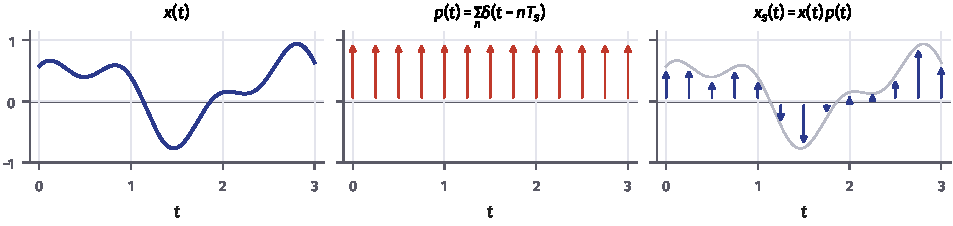
\includegraphics[width=0.9\linewidth]{tren_impulsos}
  \caption{Muestreo ideal como producto por un tren de impulsos.}
  \label{fig:tren}
\end{figure}

El tren $p(t)$ es periódico de periodo $T_s$, con coeficientes de Fourier
\[
  c_k=\frac{1}{T_s}\int_{-T_s/2}^{T_s/2}\delta(t)\,\e^{-jk\omega_st}\dd t=\frac{1}{T_s}\quad\text{para todo }k,
\]
y una señal periódica tiene transformada $\sum_k2\pi c_k\delta(\omega-k\omega_s)$. Por tanto:

\begin{propiedad}{Transformada del tren de impulsos}{tren}
  \[
    \sum_{n=-\infty}^{\infty}\delta(t-nT_s)\ \parF\ \omega_s\sum_{k=-\infty}^{\infty}\delta(\omega-k\omega_s).
  \]
  Impulsos separados $T_s$ en el tiempo se transforman en impulsos separados $\omega_s=2\pi/T_s$ en frecuencia.
\end{propiedad}

\subsection{Espectro de la señal muestreada}

Un producto en el tiempo es una convolución en frecuencia dividida por $2\pi$, y convolucionar con $\delta(\omega-k\omega_s)$ desplaza el espectro a $k\omega_s$:
\begin{equation}\label{eq:replicas}
  \boxed{X_s(j\omega)=\frac{1}{2\pi}\,X(j\omega)\conv P(j\omega)=\frac{1}{T_s}\sum_{k=-\infty}^{\infty}X\big(j(\omega-k\omega_s)\big)}
\end{equation}
El espectro de la señal muestreada es el de la original, escalado por $1/T_s$ y \emph{replicado} cada $\omega_s$ (\cref{fig:replicas}). Si las réplicas se solapan, se suman, y en la zona de solape ya no se puede saber qué parte venía de cada una: es el aliasing visto en frecuencia.

\begin{figure}[ht]
  \centering
  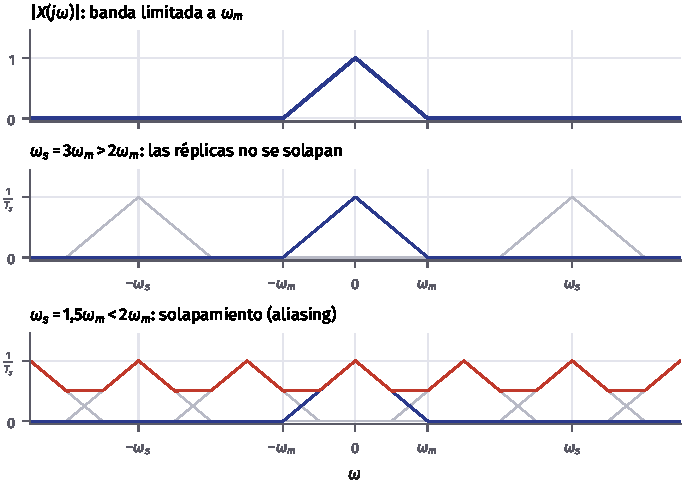
\includegraphics[width=0.62\linewidth]{espectro_replicas}
  \caption{Espectro de la señal muestreada con muestreo suficiente (arriba) e insuficiente (abajo).}
  \label{fig:replicas}
\end{figure}

\begin{definicion}{Teorema del muestreo (Nyquist–Shannon)}{nyquist}
  Sea $x(t)$ de \emph{banda limitada}, $X(j\omega)=0$ para $\abs{\omega}>\omega_m$. Si
  \[
    \omega_s>2\,\omega_m\qquad\big(f_s>2f_m\big),
  \]
  $x(t)$ queda determinada de forma única por sus muestras $x(nT_s)$.
\end{definicion}

La demostración se lee en la \cref{fig:replicas}: la réplica $k$ ocupa $[k\omega_s-\omega_m,k\omega_s+\omega_m]$, y la central y la primera no se solapan si $\omega_m<\omega_s-\omega_m$. Entonces la réplica central es $X(j\omega)/T_s$ y un filtro paso bajo la aísla (\cref{sec:reconstruccion}). La frecuencia $2f_m$ se llama \emph{tasa de Nyquist}.

La desigualdad tiene que ser estricta: $\sin(\omega_mt)$ muestreada con $\omega_s=2\omega_m$ da $\sin(\pi n)=0$ en todas las muestras. Con una componente justo en $\omega_s/2$ las dos réplicas se tocan y la amplitud y la fase de esa componente quedan indeterminadas.

\subsection{Visión continua y visión discreta}

Transformando $x_s(t)$ término a término y comparando con la DTFT de $x[n]$,
\[
  X_s(j\omega)=\sum_nx(nT_s)\,\e^{-j\omega T_sn},\qquad \Xd=\sum_nx[n]\,\e^{-j\Omega n},
\]
se ve que son la misma función con el cambio $\Omega=\omega T_s$:
\begin{equation}\label{eq:dtft-ctft}
  \Xd=X_s(j\omega)\big|_{\omega=\Omega/T_s}=\frac{1}{T_s}\sum_{k=-\infty}^{\infty}X\Big(j\,\frac{\Omega-2\pi k}{T_s}\Big).
\end{equation}

Esta relación tiene tres consecuencias que se usan continuamente:
\begin{itemize}
  \item La banda $\abs{\omega}\le\omega_s/2$ se transforma en $\abs{\Omega}\le\pi$. Toda la información de la señal muestreada está en un intervalo de anchura $2\pi$.
  \item La periodicidad $2\pi$ de la DTFT, que en el Tema~1 apareció como una propiedad matemática, \emph{es} la replicación del espectro que produce el muestreo.
  \item Si $\omega_s=2\omega_m$, la señal ocupa todo $[-\pi,\pi]$. Con \emph{sobremuestreo}, por ejemplo $\omega_s=4\omega_m$, ocupa $\abs{\Omega}\le\pi/2$ y queda una banda libre que facilita los filtros analógicos (\cref{sec:sobremuestreo}).
\end{itemize}

\begin{figure}[ht]
  \centering
  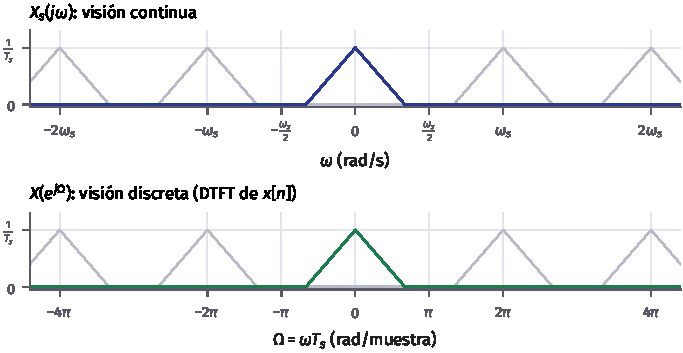
\includegraphics[width=0.8\linewidth]{vision_continua_discreta}
  \caption{El mismo espectro en función de $\omega$ (rad/s) y de $\Omega$ (rad/muestra).}
  \label{fig:vision}
\end{figure}

\begin{encodigo}
  Se muestrea a $f_s=3$\,Hz una señal $\sinc^2$ de banda $f_m=1$\,Hz y se compara $T_s\abs{X(\e^{j\Omega})}$, dibujada frente a $\omega=\Omega/T_s$, con $\abs{\Xc}$.
  \codigo{espectro_muestreado}
\end{encodigo}

\subsection{Filtro antialiasing}

Las señales reales no son de banda limitada. Una señal de duración finita tiene espectro infinito, y el ruido térmico ocupa todas las frecuencias. Lo que esté por encima de $f_s/2$ se plegará sobre la banda útil y, una vez muestreado, es imposible separarlo. Por eso, antes del conversor A/D se coloca un filtro analógico paso bajo, el \emph{filtro antialiasing}, que atenúa todo lo que hay por encima de $f_s/2$ (\cref{fig:antialiasing}).

Un filtro real no corta en seco: necesita una banda de transición. Por eso se muestrea con margen sobre la tasa de Nyquist. El audio de calidad CD ocupa hasta 20\,kHz y se muestrea a 44,1\,kHz, lo que deja una transición de 20 a 22,05\,kHz; la telefonía limita la voz a 3,4\,kHz y muestrea a 8\,kHz.

\begin{figure}[ht]
  \centering
  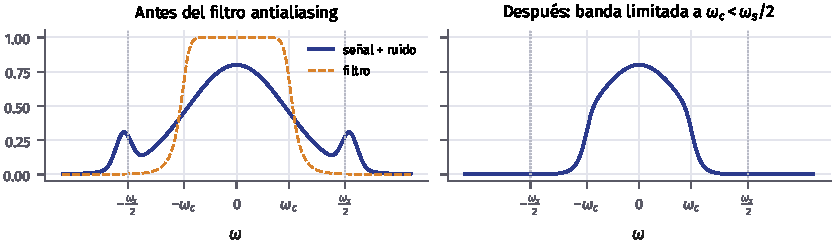
\includegraphics[width=0.8\linewidth]{antialiasing}
  \caption{El filtro antialiasing elimina la parte del espectro que se plegaría sobre la banda útil.}
  \label{fig:antialiasing}
\end{figure}

\subsection{Muestreo no ideal}

Un circuito no puede generar impulsos ideales; se muestrea con pulsos de duración $\tau$ (\cref{fig:natural}). Hay dos variantes:
\begin{itemize}
  \item \textbf{Muestreo natural}: $x_n(t)=x(t)\,p_\tau(t)$, donde $p_\tau$ es un tren de pulsos rectangulares de anchura $\tau$. Sus coeficientes de Fourier son $c_k=\frac{\tau}{T_s}\sinc\big(\frac{k\tau}{T_s}\big)$, así que
  \[
    X_n(j\omega)=\sum_kc_k\,X\big(j(\omega-k\omega_s)\big).
  \]
  Las réplicas no se deforman: solo se ponderan por $c_k$, y la central sigue siendo proporcional a $X(j\omega)$.
  \item \textbf{Muestreo de techo plano}: cada pulso mantiene el valor de la muestra, como hace un circuito de muestreo y retención (\emph{sample and hold}). Es $x_s(t)$ convolucionada con un pulso de anchura $\tau$, así que
  \[
    X_{tp}(j\omega)=X_s(j\omega)\cdot\tau\,\sinc\Big(\frac{\omega\tau}{2\pi}\Big)\e^{-j\omega\tau/2}.
  \]
  Ahora todas las réplicas, incluida la central, se multiplican por un $\sinc$: es el \emph{efecto de apertura}, que se corrige con un ecualizador o se hace despreciable con $\tau\ll T_s$. Con $\tau=T_s$ es exactamente el retenedor de orden cero de la \cref{sec:zoh}.
\end{itemize}

\begin{figure}[ht]
  \centering
  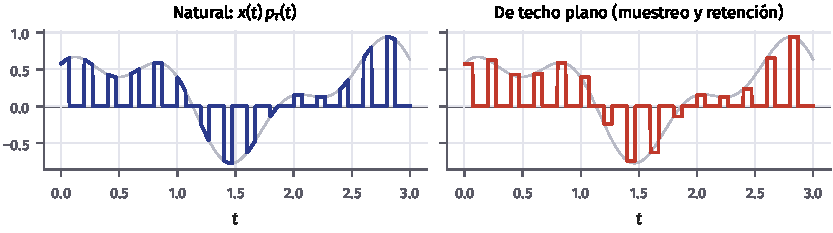
\includegraphics[width=0.8\linewidth]{muestreo_natural}
  \caption{Muestreo natural y de techo plano.}
  \label{fig:natural}
\end{figure}

\begin{flushright}\small\color{pdsgris}Ejercicios 3–5. \herramienta{html/T2\_Muestreo periódico.html} y \texttt{T2\_Muestreo natural.html}.\end{flushright}

% =====================================================================
\section{Reconstrucción}\label{sec:reconstruccion}

Reconstruir es obtener una señal continua $y(t)$ a partir de la secuencia $x[n]$ y del periodo $T_s$. En general no tiene solución única, porque infinitas señales tienen las mismas muestras. Si $x(t)$ es de banda limitada y se cumple el teorema del muestreo, la réplica central de $X_s(j\omega)$ es $X(j\omega)/T_s$ y basta un filtro que se quede con ella.

\subsection{Reconstrucción ideal}

\begin{definicion}{Filtro de reconstrucción ideal}{rec-ideal}
  \[
    H(j\omega)=T_s\,\rect\Big(\frac{\omega}{2\omega_c}\Big)=\begin{cases}T_s & \abs{\omega}\le\omega_c\\0 & \abs{\omega}>\omega_c\end{cases},\qquad \omega_m<\omega_c<\omega_s-\omega_m.
  \]
\end{definicion}

La ganancia $T_s$ compensa el factor $1/T_s$ de \eqref{eq:replicas}, y la frecuencia de corte puede ser cualquiera entre el final de la réplica central y el principio de la siguiente (\cref{fig:rec-ideal}). La elección habitual es $\omega_c=\omega_s/2$, la única posible cuando el margen es mínimo.

\begin{figure}[ht]
  \centering
  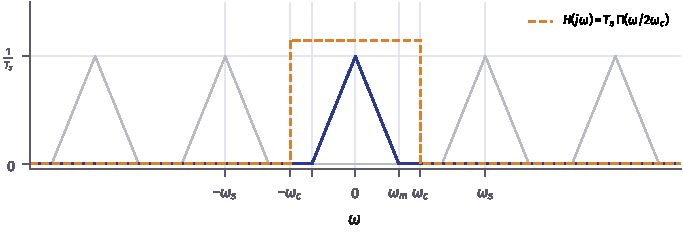
\includegraphics[width=0.7\linewidth]{reconstruccion_ideal}
  \caption{El filtro ideal de reconstrucción se queda con la réplica central.}
  \label{fig:rec-ideal}
\end{figure}

Su respuesta al impulso es
\[
  h(t)=\frac{1}{2\pi}\int_{-\omega_c}^{\omega_c}T_s\,\e^{j\omega t}\dd\omega=\frac{T_s}{\pi t}\sin(\omega_ct)=\frac{\omega_cT_s}{\pi}\Sa(\omega_ct),
\]
con $\Sa(x)=\sin x/x$. Con $\omega_c=\omega_s/2=\pi/T_s$ queda $h(t)=\sinc(t/T_s)$, con $\sinc(x)=\sin(\pi x)/(\pi x)$: vale 1 en $t=0$ y se anula en todos los demás múltiplos de $T_s$.

La salida del filtro es la convolución de $x_s(t)$ con $h(t)$, es decir, una suma de copias de $h$ centradas en cada muestra:

\begin{propiedad}{Fórmula de interpolación de Whittaker–Shannon}{interpolacion}
  Si $x(t)$ es de banda limitada a $\omega_m<\omega_s/2$,
  \[
    x(t)=\sum_{n=-\infty}^{\infty}x[n]\,\sinc\Big(\frac{t-nT_s}{T_s}\Big).
  \]
\end{propiedad}

En $t=nT_s$ solo contribuye la muestra $n$, porque las demás funciones $\sinc$ se anulan ahí; entre muestras contribuyen todas, ponderadas según su distancia (\cref{fig:sinc}).

\begin{figure}[ht]
  \centering
  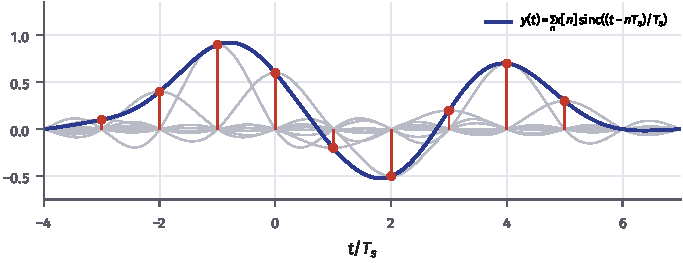
\includegraphics[width=0.8\linewidth]{interpolacion_sinc}
  \caption{Interpolación con funciones $\sinc$: la suma de las copias reproduce la señal.}
  \label{fig:sinc}
\end{figure}

\begin{ejemplo}{Elección de la frecuencia de corte}{rec-ejemplo}
  Se quiere reconstruir $x(t)=\sin(\omega_0t)$, con $\omega_0=2\pi/10$\,rad/s, a partir de sus muestras con $T_s=4$\,s. Como $\omega_s=2\pi/4=5\pi/10>2\omega_0=4\pi/10$, se cumple el teorema. Las réplicas de la sinusoide están en $\pm\omega_0+k\omega_s$; la más próxima a la central por arriba es $\omega_s-\omega_0=3\pi/10$. Cualquier $\omega_c$ con $2\pi/10<\omega_c<3\pi/10$ reconstruye exactamente la señal:
  \[
    y(t)=\sum_nx[n]\,\frac{\omega_cT_s}{\pi}\Sa\big(\omega_c(t-nT_s)\big).
  \]
  \begin{center}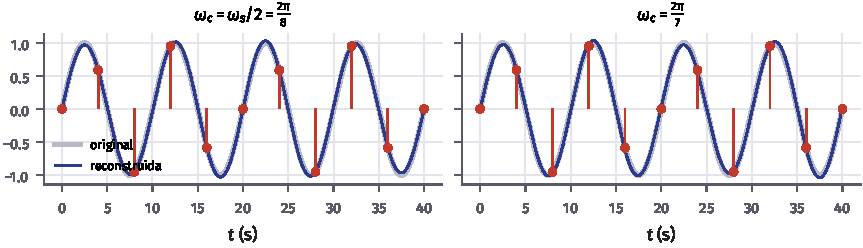
\includegraphics[width=0.8\linewidth]{ejemplo_reconstruccion}\end{center}
\end{ejemplo}

\subsection{Por qué la reconstrucción ideal no es realizable}

El filtro ideal tiene tres problemas prácticos:
\begin{itemize}
  \item Es \emph{no causal}: $h(t)\ne0$ para $t<0$, así que $y(t)$ depende de muestras futuras.
  \item Tiene \emph{duración infinita}, y $\sinc$ decae solo como $1/t$: truncar la suma deja un error apreciable.
  \item Supone una señal de banda limitada, y ninguna señal de duración finita lo es.
\end{itemize}
Además, ningún filtro analógico tiene un corte abrupto. Fuera de línea (al remuestrear audio o escalar imágenes) se usa la fórmula truncada o con ventana. En tiempo real se usan \emph{retenedores}, que interpolan con pocas muestras, seguidos de un filtro analógico de suavizado.

\begin{encodigo}
  Reconstrucción de un coseno de 2\,Hz muestreado con $T_s=0{,}1$\,s con 101 muestras. El error no es exactamente cero porque la suma está truncada.
  \codigo{reconstruccion_sinc}
\end{encodigo}

\subsection{La reconstrucción como interpolación}

Cualquier reconstrucción lineal e invariante con el desplazamiento de las muestras tiene la forma
\[
  y(t)=\sum_nx[n]\,h(t-nT_s)\quad\Longleftrightarrow\quad Y(j\omega)=H(j\omega)\,X_s(j\omega).
\]
La \emph{función de interpolación} $h(t)$ dice cuánto contribuye cada muestra según su distancia al instante $t$, y su transformada $H(j\omega)$ dice cuánto se deforma la réplica central y cuánto se atenúan las demás. El filtro ideal es el caso $h=\sinc$; los retenedores usan funciones más cortas (\cref{fig:ret-h}).

\begin{figure}[ht]
  \centering
  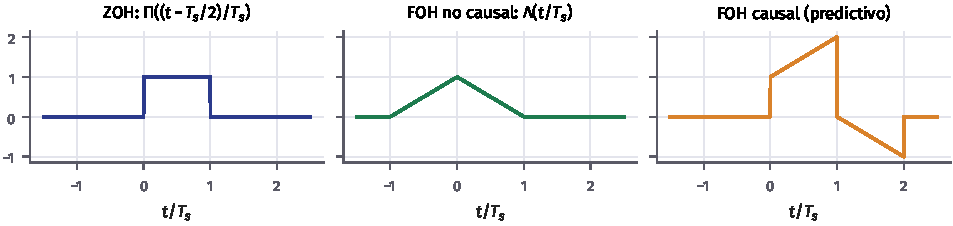
\includegraphics[width=0.9\linewidth]{retenedores_h}
  \caption{Funciones de interpolación de los retenedores de orden cero y uno.}
  \label{fig:ret-h}
\end{figure}

\subsection{Retenedor de orden cero}\label{sec:zoh}

El retenedor de orden cero (ZOH, \emph{zero-order hold}) mantiene cada muestra hasta la siguiente: $y(t)=x[n]$ para $nT_s\le t<(n+1)T_s$. Su función de interpolación es un pulso de anchura $T_s$ que empieza en el origen:
\[
  h_0(t)=\rect\Big(\frac{t-T_s/2}{T_s}\Big).
\]
Su transformada es la de un pulso centrado, $T_s\sinc(\omega/\omega_s)$, retrasada $T_s/2$:
\begin{equation}\label{eq:zoh}
  \boxed{H_0(j\omega)=T_s\,\e^{-j\omega T_s/2}\,\sinc\Big(\frac{\omega}{\omega_s}\Big)=T_s\,\e^{-j\omega T_s/2}\,\Sa\Big(\frac{\omega T_s}{2}\Big)}
\end{equation}

\begin{nota}[Errata frecuente]
  El retardo del ZOH es $\e^{-j\omega T_s/2}$, con signo negativo: el pulso está a la \emph{derecha} del origen. Con signo positivo el retenedor sería anticipativo.
\end{nota}

El ZOH es causal y muy sencillo: es lo que hace un conversor D/A al mantener su salida hasta el siguiente código. Pero no es un buen filtro de reconstrucción (\cref{fig:zoh}):
\begin{itemize}
  \item \textbf{Atenúa la banda útil}. En $\omega_s/2$, $\abs{H_0}/T_s=\sinc(1/2)=2/\pi$, unos $-3{,}9$\,dB. Para audio a 44,1\,kHz, en 20\,kHz la atenuación es de $3{,}2$\,dB.
  \item \textbf{No elimina las réplicas}, solo las atenúa como $1/\omega$. La primera imagen de un tono de 20\,kHz, en 24,1\,kHz, sale solo $4{,}8$\,dB por debajo.
  \item Introduce un \textbf{retardo} de media muestra.
\end{itemize}

\begin{figure}[ht]
  \centering
  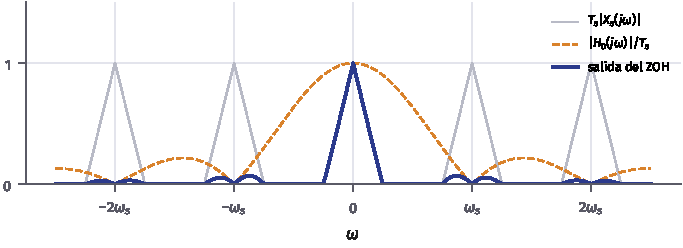
\includegraphics[width=0.6\linewidth]{zoh_espectro}
  \caption{Módulo de la respuesta del ZOH frente al filtro ideal.}
  \label{fig:zoh}
\end{figure}

\subsection{Retenedor de orden uno}

El retenedor de orden uno (FOH, \emph{first-order hold}) une las muestras con segmentos rectos. Hay dos versiones:

\paragraph{FOH no causal (interpolación lineal).} Entre $nT_s$ y $(n+1)T_s$,
\[
  y(t)=x[n]+\big(x[n+1]-x[n]\big)\frac{t-nT_s}{T_s}.
\]
La función de interpolación es un triángulo de base $2T_s$ centrado en el origen, que es la convolución de dos pulsos de anchura $T_s$ dividida por $T_s$:
\[
  h_1(t)=\tri\Big(\frac{t}{T_s}\Big)=\frac{1}{T_s}\,\rect\Big(\frac{t}{T_s}\Big)\conv\rect\Big(\frac{t}{T_s}\Big)
  \quad\Longrightarrow\quad
  \boxed{H_1(j\omega)=T_s\,\sinc^2\Big(\frac{\omega}{\omega_s}\Big)}
\]
Es real y positiva (fase nula) y las réplicas caen como $1/\omega^2$. Usa la muestra siguiente, así que no es causal; retrasándolo una muestra se vuelve causal, con $H=T_s\e^{-j\omega T_s}\sinc^2(\omega/\omega_s)$, a costa de un retardo $T_s$.

\paragraph{FOH causal (predictivo).} Prolonga la recta que pasa por las dos últimas muestras:
\[
  y(t)=x[n]+\big(x[n]-x[n-1]\big)\frac{t-nT_s}{T_s},\qquad nT_s\le t<(n+1)T_s.
\]
La contribución de una muestra aislada es una rampa ascendente seguida de una descendente,
\[
  h(t)=\begin{cases}1+t/T_s & 0\le t<T_s\\ 1-t/T_s & T_s\le t<2T_s\\ 0 & \text{en otro caso}\end{cases}
  \qquad\Longrightarrow\qquad
  H(j\omega)=T_s\,(1+j\omega T_s)\,\e^{-j\omega T_s}\,\sinc^2\Big(\frac{\omega}{\omega_s}\Big).
\]
El factor $1+j\omega T_s$ amplifica las altas frecuencias: la salida tiene saltos en cada instante de muestreo y sobrepasa la señal cuando cambia la pendiente (\cref{fig:ret-t}).

\begin{figure}[ht]
  \centering
  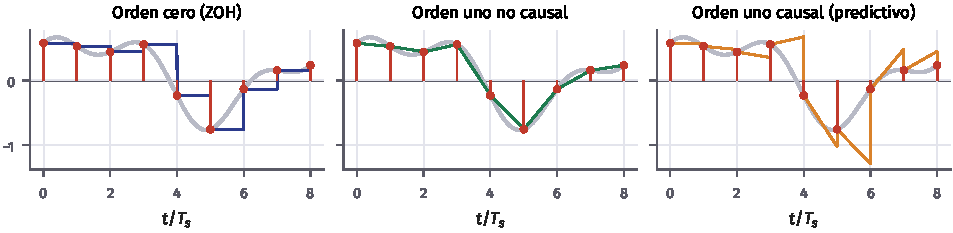
\includegraphics[width=\linewidth]{retenedores_tiempo}
  \caption{Los tres retenedores aplicados a la misma secuencia.}
  \label{fig:ret-t}
\end{figure}

\subsection{Comparación y conversión D/A}

El \cref{tab:retenedores} y la \cref{fig:ret-f} resumen los retenedores. Ninguno reconstruye exactamente: deforman la banda útil y dejan pasar parte de las réplicas. Cuanto mayor es el orden, mejor atenúan las réplicas, pero necesitan más muestras y más retardo. Una cota útil del error para una señal suave: el ZOH comete un error de hasta $\max\abs{x'}\,T_s$, y la interpolación lineal, de hasta $\max\abs{x''}\,T_s^2/8$.

\begin{table}[ht]
  \centering
  \renewcommand{\arraystretch}{1.3}
  \begin{tabular}{@{}llll@{}}
    \toprule
    & $h(t)$ & $\abs{H(j\omega)}/T_s$ & Causal\\\midrule
    Ideal & $\sinc(t/T_s)$ & $\rect(\omega/\omega_s)$ & No\\
    ZOH & $\rect\big(\frac{t-T_s/2}{T_s}\big)$ & $\abs{\sinc(\omega/\omega_s)}$ & Sí\\
    FOH no causal & $\tri(t/T_s)$ & $\sinc^2(\omega/\omega_s)$ & No (sí con retardo $T_s$)\\
    FOH predictivo & dos rampas en $[0,2T_s)$ & $\abs{1+j\omega T_s}\sinc^2(\omega/\omega_s)$ & Sí\\\bottomrule
  \end{tabular}
  \caption{Comparación de los métodos de reconstrucción.}
  \label{tab:retenedores}
\end{table}

\begin{figure}[ht]
  \centering
  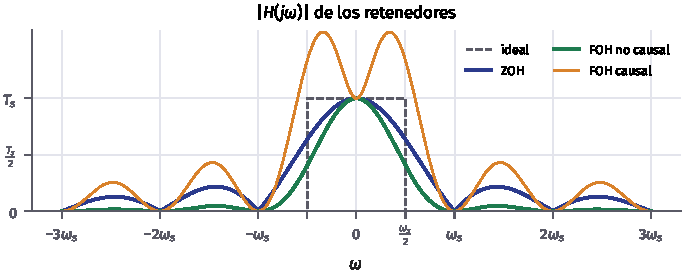
\includegraphics[width=0.7\linewidth]{retenedores_frecuencia}
  \caption{Respuesta en frecuencia de los retenedores.}
  \label{fig:ret-f}
\end{figure}

Un conversor D/A real combina las piezas: una \emph{compensación} digital con respuesta $1/\sinc(\omega/\omega_s)$ en la banda útil corrige la caída del ZOH; el conversor mantiene cada valor (ZOH); y un \emph{filtro de suavizado} analógico elimina las réplicas que el ZOH deja pasar. Con sobremuestreo (\cref{sec:sobremuestreo}) las réplicas se alejan y ese filtro puede ser muy sencillo.

\begin{encodigo}
  Reconstrucción de una sinusoide con diez muestras por periodo con ZOH y FOH no causal. El error máximo del ZOH es $0{,}59$ y el del FOH, $0{,}05$.
  \codigo{retenedores}
\end{encodigo}

\begin{flushright}\small\color{pdsgris}Ejercicios 7–10. \herramienta{html/T2\_Reconstrucción.html} y \texttt{T2\_Retenedores.html}.\end{flushright}

% =====================================================================
\section{Cuantificación y codificación}\label{sec:cuantificacion}

El muestreo discretiza el tiempo, pero la amplitud de $x[n]$ sigue siendo \emph{continua}. Un procesador solo puede almacenar números con un número finito de bits, así que cada muestra se aproxima por uno de un conjunto finito de valores. A diferencia del muestreo, esta aproximación siempre pierde información.

\subsection{Cuantificador uniforme}

\begin{definicion}{Cuantificación}{cuantificacion}
  La \emph{cuantificación} asigna a cada muestra $x[n]$ uno de $L$ valores permitidos, los \emph{niveles de cuantificación}:
  \[
    x_q[n]=Q\big[x[n]\big].
  \]
  En un cuantificador \emph{uniforme} los niveles están separados por un \emph{escalón} o \emph{resolución} constante $\Delta$. La diferencia $e[n]=x_q[n]-x[n]$ es el \emph{error de cuantificación}.
\end{definicion}

Con $b$ bits hay $L=2^b$ niveles. Si la entrada está en el margen $[-V,V)$, de \emph{fondo de escala} $FS=2V$,
\begin{equation}\label{eq:delta}
  \Delta=\frac{FS}{2^b}=\frac{2V}{2^b}.
\end{equation}
Es el convenio de los conversores A/D, donde $\Delta$ es el valor del bit menos significativo (1~LSB). En el margen bipolar los niveles son $k\Delta$ con $k=-2^{b-1},\dots,2^{b-1}-1$: hay un nivel en cero y el margen es ligeramente asimétrico.

\begin{nota}[Otro convenio]
  Algunos textos colocan el primer y el último nivel exactamente en los extremos del intervalo $[x_{\min},x_{\max}]$, y entonces $\Delta=\frac{x_{\max}-x_{\min}}{L-1}$. Las dos definiciones difieren en un nivel y dan las mismas conclusiones para $L$ grande. En este curso se usa \eqref{eq:delta}.
\end{nota}

Si la entrada se sale del margen, el cuantificador \emph{satura}: devuelve el nivel extremo y el error deja de estar acotado por $\Delta$. Por eso el margen del conversor debe ajustarse a la señal, sin quedarse corto (saturación) ni largo (se desperdician niveles).

\subsection{Redondeo y truncamiento}

Hay dos formas habituales de elegir el nivel (\cref{fig:cuantificador}):
\begin{itemize}
  \item \textbf{Redondeo}: el nivel más próximo, $Q[x]=\Delta\,\operatorname{round}(x/\Delta)$. El error está en $-\Delta/2\le e<\Delta/2$ y tiene media nula.
  \item \textbf{Truncamiento}: el nivel inmediatamente inferior, $Q[x]=\Delta\lfloor x/\Delta\rfloor$. El error está en $-\Delta<e\le0$: tiene un sesgo de $-\Delta/2$.
\end{itemize}

\begin{figure}[ht]
  \centering
  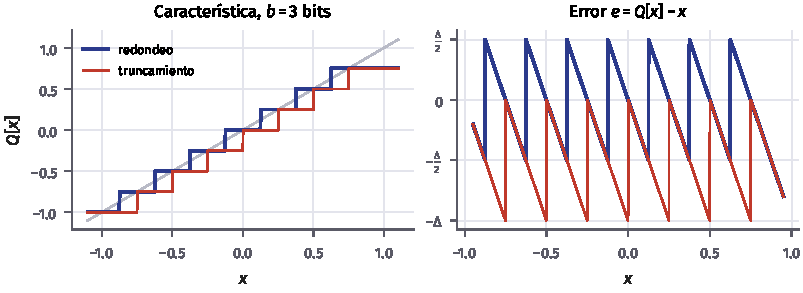
\includegraphics[width=0.9\linewidth]{cuantificador}
  \caption{Característica de un cuantificador de 3 bits y error de cuantificación.}
  \label{fig:cuantificador}
\end{figure}

\begin{ejemplo}{Cuantificar $x[n]=0{,}9^n$}{09n}
  Para representar exactamente los diez primeros valores ($n=0,\dots,9$) hace falta $\Delta=10^{-9}$, porque $0{,}9^9=0{,}387420489$ tiene nueve decimales. Con un decimal, $\Delta=0{,}1$:
  \begin{center}
    \small
    \begin{tabular}{@{}rlllll@{}}
      \toprule
      & & \multicolumn{2}{c}{$x_q[n]$} & \multicolumn{2}{c}{$e[n]$}\\\cmidrule(lr){3-4}\cmidrule(l){5-6}
      $n$ & $x[n]$ & truncado & redondeado & truncado & redondeado\\\midrule
      0 & 1 & 1,0 & 1,0 & 0 & 0\\
      1 & 0,9 & 0,9 & 0,9 & 0 & 0\\
      2 & 0,81 & 0,8 & 0,8 & $-0{,}01$ & $-0{,}01$\\
      3 & 0,729 & 0,7 & 0,7 & $-0{,}029$ & $-0{,}029$\\
      4 & 0,6561 & 0,6 & 0,7 & $-0{,}0561$ & $0{,}0439$\\
      5 & 0,59049 & 0,5 & 0,6 & $-0{,}09049$ & $0{,}00951$\\
      6 & 0,531441 & 0,5 & 0,5 & $-0{,}031441$ & $-0{,}031441$\\
      7 & 0,4782969 & 0,4 & 0,5 & $-0{,}0782969$ & $0{,}0217031$\\
      8 & 0,43046721 & 0,4 & 0,4 & $-0{,}03046721$ & $-0{,}03046721$\\
      9 & 0,387420489 & 0,3 & 0,4 & $-0{,}087420489$ & $0{,}012579511$\\\bottomrule
    \end{tabular}
  \end{center}
  Truncando, todos los errores son negativos y de hasta $-0{,}09$; redondeando, cambian de signo y no superan $0{,}05$ en valor absoluto.
\end{ejemplo}

\subsection{Ruido de cuantificación}

El error de cuantificación es una función determinista de la señal, pero si la señal es activa (cruza muchos niveles entre muestra y muestra) y no satura, se comporta como un ruido aditivo (\cref{fig:error}):
\[
  x_q[n]=x[n]+e[n],
\]
con $e[n]$ uniformemente distribuido en $[-\Delta/2,\Delta/2)$, incorrelado con $x[n]$ y blanco (sus muestras son independientes entre sí). Su media es nula y su potencia es
\begin{equation}\label{eq:ruido}
  \boxed{\sigma_e^2=\frac{1}{\Delta}\int_{-\Delta/2}^{\Delta/2}e^2\dd e=\frac{\Delta^2}{12}}
\end{equation}
Con truncamiento la varianza es la misma, pero la media es $-\Delta/2$. El modelo falla si la señal es lenta o pequeña frente a $\Delta$: entonces el error se parece a la propia señal y aparece como distorsión armónica. Las herramientas para describir señales aleatorias se estudian en el Tema~6.

\begin{figure}[ht]
  \centering
  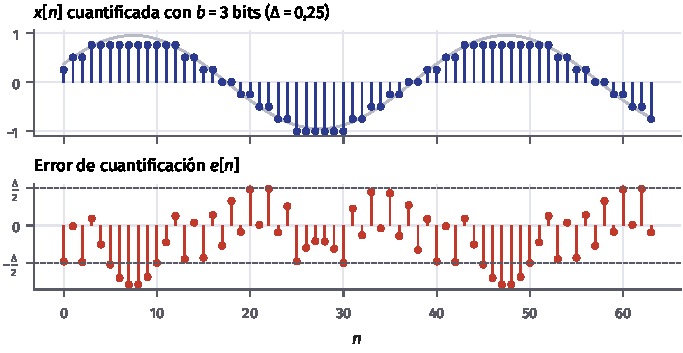
\includegraphics[width=0.65\linewidth]{error_cuantificacion}
  \caption{Señal cuantificada con 3 bits y su error de cuantificación.}
  \label{fig:error}
\end{figure}

La calidad de la cuantificación se mide con la \emph{relación señal a ruido de cuantificación},
\[
  \mathrm{SQNR}=10\log_{10}\frac{P_x}{\sigma_e^2}\ \text{dB}.
\]
Para una sinusoide que ocupa todo el margen, de amplitud $V$, $P_x=V^2/2$, y con \eqref{eq:delta} y \eqref{eq:ruido}:
\begin{equation}\label{eq:sqnr}
  \boxed{\mathrm{SQNR}=10\log_{10}\frac{V^2/2}{(2V)^2/(12\cdot2^{2b})}=10\log_{10}\Big(\frac32\,2^{2b}\Big)\approx6{,}02\,b+1{,}76\ \text{dB}}
\end{equation}
Cada bit añade unos 6\,dB (\cref{fig:sqnr}). Un CD, con 16 bits, alcanza unos 98\,dB. La fórmula supone que la señal aprovecha todo el margen: si su amplitud es $V/10$, la SQNR baja 20\,dB, lo que equivale a perder más de tres bits.

\begin{figure}[ht]
  \centering
  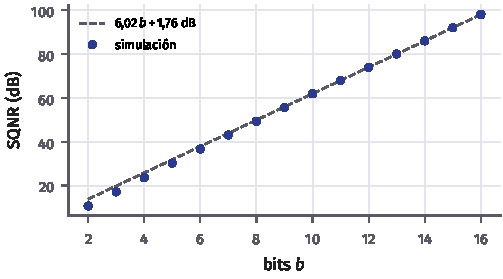
\includegraphics[width=0.5\linewidth]{sqnr_bits}
  \caption{SQNR medida y teórica en función del número de bits.}
  \label{fig:sqnr}
\end{figure}

\begin{encodigo}
  Cuantificación por redondeo con 8 bits de una sinusoide de amplitud $0{,}99\,V$. La varianza del error coincide con $\Delta^2/12$ y la SQNR medida, $49{,}7$\,dB, con los $49{,}9$\,dB de \eqref{eq:sqnr}.
  \codigo{cuantificacion}
\end{encodigo}

\subsection{Codificación}

La codificación asigna a cada nivel una palabra binaria. Con $b$ bits hay $2^b$ palabras, así que para $L$ niveles hace falta
\[
  2^b\ge L\quad\Longrightarrow\quad b\ge\log_2L.
\]
Por ejemplo, 6 niveles necesitan $b\ge\log_26\approx2{,}585$, es decir, 3 bits (y sobran dos palabras).

Para un margen bipolar, con niveles $k\Delta$, se usan sobre todo dos códigos (\cref{tab:codigos}): el \emph{binario desplazado}, que codifica $k+2^{b-1}$ en binario natural y es el que entregan muchos conversores, y el \emph{complemento a dos}, que es el de la aritmética entera de los procesadores. Pasar de uno a otro es tan sencillo como invertir el bit más significativo.

\begin{table}[ht]
  \centering
  \begin{tabular}{@{}rrcc@{}}
    \toprule
    $k$ & $x_q=k\Delta$ & binario desplazado & complemento a dos\\\midrule
    3 & $3\Delta$ & 111 & 011\\
    2 & $2\Delta$ & 110 & 010\\
    1 & $\Delta$ & 101 & 001\\
    0 & 0 & 100 & 000\\
    $-1$ & $-\Delta$ & 011 & 111\\
    $-2$ & $-2\Delta$ & 010 & 110\\
    $-3$ & $-3\Delta$ & 001 & 101\\
    $-4$ & $-4\Delta$ & 000 & 100\\\bottomrule
  \end{tabular}
  \caption{Códigos de un cuantificador bipolar de 3 bits.}
  \label{tab:codigos}
\end{table}

\subsection{Parámetros de un conversor A/D}

Un conversor A/D se describe por:
\begin{itemize}
  \item Su \textbf{resolución} $b$ y su \textbf{tensión de referencia} $V_{\text{ref}}$. Con un margen unipolar $[0,V_{\text{ref}})$, $1\,\text{LSB}=\Delta=V_{\text{ref}}/2^b$.
  \item Su \textbf{rango dinámico}: el cociente entre la mayor y la menor amplitud que distingue,
  \[
    \mathrm{DR}=20\log_{10}\frac{V_{\text{ref}}}{\Delta}=20\log_{10}2^b\approx6{,}02\,b\ \text{dB}.
  \]
  Ojo: «rango dinámico» designa a veces el intervalo de valores de la entrada. Aquí lo reservamos para el cociente en decibelios y llamamos \emph{margen} al intervalo.
  \item Su \textbf{frecuencia de muestreo} máxima, ligada al tiempo de conversión.
  \item Su \textbf{arquitectura}: \emph{flash} (muy rápida, pocos bits), de aproximaciones sucesivas (SAR, el compromiso habitual en microcontroladores) o sigma-delta (muchos bits gracias al sobremuestreo, \cref{sec:sobremuestreo}).
\end{itemize}

\begin{ejemplo}{Conversor de un microcontrolador}{adc}
  Un conversor de 10 bits con $V_{\text{ref}}=3{,}3$\,V tiene $\Delta=3{,}3/1024\approx3{,}22$\,mV y $\mathrm{DR}\approx60{,}2$\,dB. Para una sinusoide que ocupe todo el margen, la SQNR es de unos 62\,dB. Si se quiere distinguir variaciones de $0{,}1$\,mV, hacen falta $b\ge\log_2(3{,}3/10^{-4})\approx15{,}01$, es decir, 16 bits.
\end{ejemplo}

\begin{flushright}\small\color{pdsgris}Ejercicios 11–13.\end{flushright}

% =====================================================================
\section{Muestreo de señales discretas}\label{sec:discreto}

Muchas veces hay que cambiar la frecuencia de muestreo de una señal que ya es discreta: pasar audio de 48\,kHz a los 8\,kHz de la telefonía, o de los 44,1\,kHz del CD a los 48\,kHz del vídeo; cambiar el tamaño de una imagen; o procesar a la menor frecuencia posible para ahorrar cálculo. Volver al dominio analógico y muestrear de nuevo añadiría ruido y coste. Todo lo visto para señales continuas tiene su versión discreta: réplicas, aliasing y filtros (\cref{fig:diezmado-t}).

\begin{figure}[ht]
  \centering
  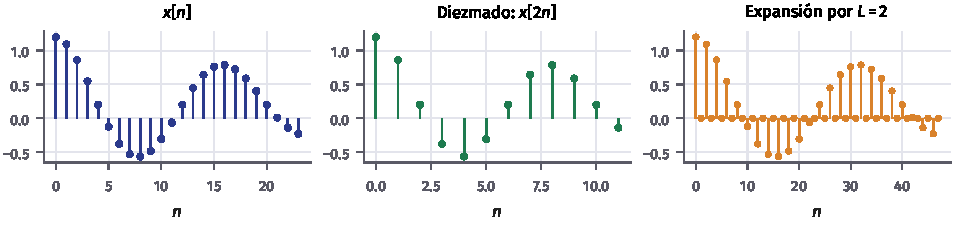
\includegraphics[width=\linewidth]{diezmado_tiempo}
  \caption{Una secuencia, su versión diezmada por 2 y su versión expandida por 2.}
  \label{fig:diezmado-t}
\end{figure}

\subsection{Muestreo de una secuencia}

Muestrear una secuencia con periodo $N$ es conservar una de cada $N$ muestras y poner a cero las demás:
\[
  x_p[n]=x[n]\,p[n],\qquad p[n]=\sum_{k=-\infty}^{\infty}\delta[n-kN].
\]
El tren $p[n]$ es periódico de periodo $N$, con desarrollo en serie de Fourier discreta
\[
  p[n]=\frac1N\sum_{k=0}^{N-1}\e^{j2\pi kn/N}.
\]
Multiplicar por $\e^{j2\pi kn/N}$ desplaza el espectro $2\pi k/N$, así que

\begin{propiedad}{Espectro de una secuencia muestreada}{muestreo-discreto}
  \[
    X_p(\e^{j\Omega})=\frac{1}{N}\sum_{k=0}^{N-1}X\big(\e^{j(\Omega-2\pi k/N)}\big).
  \]
\end{propiedad}

Es la versión discreta de \eqref{eq:replicas}: aparecen $N-1$ réplicas separadas $\Omega_s=2\pi/N$. Si $x[n]$ tiene banda limitada a $\Omega_m$, no se solapan cuando $\Omega_m<\pi/N$, y entonces $x[n]$ se recupera de $x_p[n]$ con un filtro paso bajo ideal de ganancia $N$ y corte $\pi/N$.

\subsection{Diezmado}

Las muestras nulas de $x_p[n]$ no aportan nada; eliminarlas es \emph{diezmar} (o submuestrear) por un factor $M$:
\[
  x_d[n]=x[nM]=x_p[nM].
\]
La nueva frecuencia de muestreo es $f_s/M$. Como $X_d(\e^{j\Omega})=\sum_nx_p[nM]\e^{-j\Omega n}=X_p(\e^{j\Omega/M})$, el espectro se \emph{expande} por $M$:

\begin{propiedad}{Diezmado}{diezmado}
  \[
    X_d(\e^{j\Omega})=\frac1M\sum_{k=0}^{M-1}X\big(\e^{j(\Omega-2\pi k)/M}\big).
  \]
  No hay aliasing si $\Omega_m<\pi/M$.
\end{propiedad}

El resultado sigue siendo periódico de periodo $2\pi$, como debe ser la DTFT de cualquier secuencia: la réplica $k$ queda centrada en $2\pi k$ (\cref{fig:diezmado-f}). Es lo esperable de \eqref{eq:omega}: con la nueva frecuencia de muestreo, cada frecuencia en hercios corresponde a una frecuencia discreta $M$ veces mayor.

\begin{figure}[ht]
  \centering
  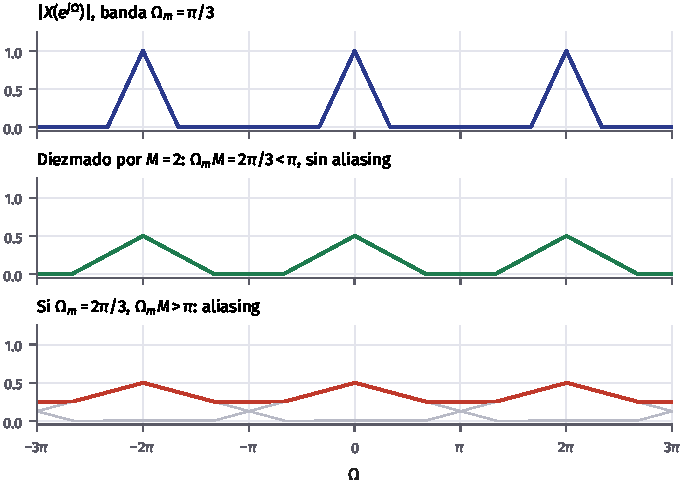
\includegraphics[width=0.75\linewidth]{diezmado_espectro}
  \caption{Diezmado por $M=2$ sin aliasing (centro) y con aliasing (abajo).}
  \label{fig:diezmado-f}
\end{figure}

Si $x[n]$ ocupa más de $\pi/M$, antes de diezmar hay que filtrarla con un paso bajo de ganancia 1 y corte $\pi/M$ (\cref{fig:diezmador}). Es el mismo papel que el filtro antialiasing analógico: se pierde la banda alta, pero no se mezcla con la baja. El filtro trabaja a la frecuencia alta, aunque solo hace falta calcular una de cada $M$ salidas.

\begin{figure}[ht]
  \centering
  \begin{tikzpicture}[node distance=1.2cm]
    \node (x) {$x[n]$};
    \node[bloque, right=of x] (h) {$H_d(\e^{j\Omega})$\\corte $\pi/M$};
    \node[bloque, right=of h] (m) {$\downarrow M$};
    \node[right=of m] (y) {$y[n]$};
    \draw[flecha] (x) -- (h); \draw[flecha] (h) -- (m); \draw[flecha] (m) -- (y);
  \end{tikzpicture}
  \caption{Diezmador con filtro antialiasing.}
  \label{fig:diezmador}
\end{figure}

\begin{ejemplo}{De 48\,kHz a 8\,kHz}{48a8}
  El factor es $M=6$. El filtro corta en $\pi/6$, que a $f_s=48$\,kHz equivale a $\frac{\pi/6}{2\pi}\cdot48=4$\,kHz: justo la frecuencia de Nyquist de la señal de salida.
\end{ejemplo}

\subsection{Expansión e interpolación}

Para aumentar la frecuencia de muestreo por un factor entero $L$, primero se insertan $L-1$ ceros entre cada par de muestras (\emph{expansión}):
\[
  x_e[n]=\begin{cases}x[n/L] & n=0,\pm L,\pm2L,\dots\\0 & \text{en otro caso}\end{cases}
  \qquad\Longrightarrow\qquad
  X_e(\e^{j\Omega})=\sum_kx[k]\e^{-j\Omega kL}=X(\e^{j\Omega L}).
\]
El espectro se \emph{comprime} por $L$ y en $[-\pi,\pi]$ aparecen $L-1$ copias adicionales, las \emph{imágenes} (\cref{fig:expansion}). Un \emph{filtro de interpolación} paso bajo de ganancia $L$ y corte $\pi/L$ las elimina y «rellena» los ceros. La ganancia $L$ compensa los ceros insertados: el valor medio de $x_e[n]$ es $1/L$ del de $x[n]$.

\begin{figure}[ht]
  \centering
  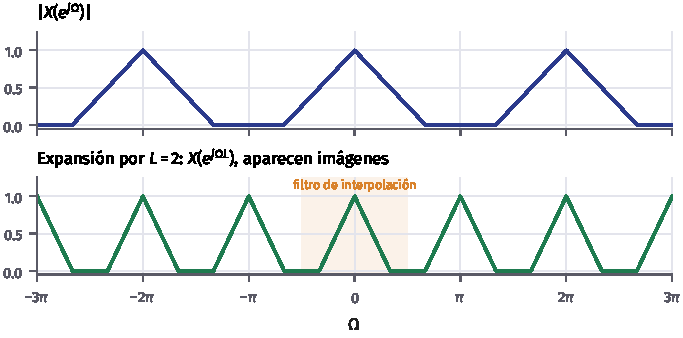
\includegraphics[width=0.75\linewidth]{expansion_espectro}
  \caption{Expansión por $L=2$: el espectro se comprime y aparecen imágenes.}
  \label{fig:expansion}
\end{figure}

Con el filtro ideal, cuya respuesta al impulso es $h[n]=\sinc(n/L)$, la salida es la interpolación de banda limitada de las muestras,
\[
  y[n]=\sum_kx[k]\,\sinc\Big(\frac{n-kL}{L}\Big),
\]
que es la fórmula de Whittaker–Shannon evaluada en los nuevos instantes; en particular, $y[kL]=x[k]$. Con filtros más sencillos se obtienen los retenedores discretos: repetir cada muestra $L$ veces ($h[n]=1$ para $0\le n<L$, orden cero) o interpolar linealmente ($h[n]=\tri(n/L)$, orden uno).

\subsection{Cambio de frecuencia por un factor racional}

Para cambiar la frecuencia por un factor racional $L/M$ se interpola por $L$ y después se diezma por $M$ (\cref{fig:racional}). En ese orden no se pierde banda innecesariamente, y los dos filtros, el de interpolación y el antialiasing, se funden en uno solo con ganancia $L$ y corte $\min(\pi/L,\pi/M)$.

\begin{figure}[ht]
  \centering
  \begin{tikzpicture}[node distance=1.0cm]
    \node (x) {$x[n]$};
    \node[bloque, right=of x] (l) {$\uparrow L$};
    \node[bloque, right=of l] (h) {Paso bajo, ganancia $L$\\corte $\min(\pi/L,\pi/M)$};
    \node[bloque, right=of h] (m) {$\downarrow M$};
    \node[right=of m] (y) {$y[n]$};
    \draw[flecha] (x) -- (l); \draw[flecha] (l) -- (h); \draw[flecha] (h) -- (m); \draw[flecha] (m) -- (y);
  \end{tikzpicture}
  \caption{Cambio de frecuencia de muestreo por un factor $L/M$.}
  \label{fig:racional}
\end{figure}

\begin{ejemplo}{De 44,1\,kHz a 48\,kHz}{cd}
  $48\,000/44\,100=160/147$, que ya es irreducible. Se interpola por $L=160$, lo que da una frecuencia intermedia de $7{,}056$\,MHz, se filtra con corte $\pi/160$ y se diezma por $M=147$. Calcular directamente así sería muy caro; en la práctica se usan estructuras \emph{polifásicas}, que no calculan las muestras que se van a descartar ni multiplican por los ceros insertados.
\end{ejemplo}

\begin{encodigo}
  Diezmado por 4 con filtro antialiasing incluido (\texttt{decimate}) y cambio de 44,1 a 48\,kHz con una estructura polifásica (\texttt{resample\_poly} en Python, \texttt{resample} en Matlab).
  \codigo{cambio_frecuencia}
\end{encodigo}

\subsection{Conversores con sobremuestreo}\label{sec:sobremuestreo}

Los conversores modernos muestrean mucho más deprisa de lo que exige el teorema y ajustan la frecuencia en digital:
\begin{itemize}
  \item \textbf{A/D}: se muestrea a $Kf_s$ y se diezma por $K$. El filtro antialiasing analógico puede ser muy suave, porque su transición va de $f_m$ a $Kf_s-f_m$; el filtro abrupto lo hace el diezmador digital. Además, el ruido de cuantificación, de potencia $\Delta^2/12$, se reparte uniformemente en $[-\pi,\pi]$ y el filtro del diezmador solo deja pasar la fracción $1/K$:
  \[
    \mathrm{SQNR}\approx6{,}02\,b+1{,}76+10\log_{10}K\ \text{dB}.
  \]
  Cada factor 4 de sobremuestreo gana unos 6\,dB, es decir, un bit.
  \item \textbf{D/A}: se interpola por $K$ antes del conversor. Las imágenes se alejan hasta $Kf_s$, el filtro de suavizado es sencillo y la caída del ZOH en la banda útil es casi nula.
\end{itemize}
Los conversores \emph{sigma-delta} van más allá: un lazo de realimentación \emph{conforma} el ruido de cuantificación para empujarlo fuera de la banda útil, de modo que con un cuantificador de un solo bit a varios megahercios se logran de 16 a 24 bits efectivos en la banda de audio.

\begin{flushright}\small\color{pdsgris}Ejercicios 14–16.\end{flushright}

% =====================================================================
\section*{Resumen del tema}
\addcontentsline{toc}{section}{Resumen del tema}

\begin{itemize}
  \item Muestreo periódico: $x[n]=x(nT_s)$; frecuencia discreta $\Omega=\omega T_s=2\pi f/f_s$.
  \item Las frecuencias $\pm\omega_0+k\omega_s$ dan las mismas muestras (aliasing). El alias fundamental es el único con $\abs{\omega}\le\omega_s/2$.
  \item Espectro de la señal muestreada: $X_s(j\omega)=\frac1{T_s}\sum_kX(j(\omega-k\omega_s))$, y $\Xd=X_s(j\Omega/T_s)$.
  \item Teorema del muestreo: una señal de banda limitada a $\omega_m$ queda determinada por sus muestras si $\omega_s>2\omega_m$. En la práctica, filtro antialiasing y margen.
  \item Reconstrucción ideal: filtro $T_s\rect(\omega/2\omega_c)$ e interpolación con $\sinc$. No es causal ni realizable.
  \item Retenedores: ZOH, $H_0=T_s\e^{-j\omega T_s/2}\sinc(\omega/\omega_s)$; FOH, $H_1=T_s\sinc^2(\omega/\omega_s)$. Un D/A real usa ZOH, compensación y filtro de suavizado.
  \item Cuantificación uniforme: $\Delta=FS/2^b$; error uniforme de potencia $\Delta^2/12$; $\mathrm{SQNR}\approx6{,}02\,b+1{,}76$\,dB. Codificar $L$ niveles requiere $b\ge\log_2L$ bits.
  \item Diezmado: $X_d=\frac1M\sum_kX(\e^{j(\Omega-2\pi k)/M})$, sin aliasing si $\Omega_m<\pi/M$. Expansión: $X_e=X(\e^{j\Omega L})$, con imágenes que elimina un filtro de ganancia $L$ y corte $\pi/L$. Cambio racional: interpolar, filtrar y diezmar.
  \item El sobremuestreo simplifica los filtros analógicos y mejora la SQNR en $10\log_{10}K$\,dB.
\end{itemize}

% =====================================================================
\section*{Bibliografía}
\addcontentsline{toc}{section}{Bibliografía}

\begin{itemize}
  \item F.~T. Ulaby y A.~E. Yagle, \emph{Signals and Systems: Theory and Applications}, 2.ª ed. Michigan Publishing Services, 2024. Capítulo de aplicaciones de la transformada de Fourier, apartados de muestreo. Descarga libre en\\ \url{https://services.publishing.umich.edu/Books/S/Signals-and-Systems}.
  \item A.~V. Oppenheim y A.~S. Willsky, \emph{Señales y sistemas}, 2.ª ed. Prentice Hall, 1997. Capítulo 7, la referencia para el muestreo, la reconstrucción y el muestreo de señales discretas.
  \item J.~G. Proakis y D.~G. Manolakis, \emph{Tratamiento digital de señales}, 4.ª ed. Pearson Prentice Hall, 2007. Capítulos 1 (conversión A/D y D/A), 6 (muestreo y reconstrucción) y 11 (cambio de frecuencia de muestreo).
  \item A.~V. Oppenheim y R.~W. Schafer, \emph{Tratamiento de señales en tiempo discreto}, 3.ª ed. Pearson, 2011. Capítulo 4, con el diezmado, la interpolación, el sobremuestreo y el ruido de cuantificación.
\end{itemize}

\end{document}
